
% 
% Example SDSU Mathematics/Physics LaTeX Thesis.
% Lines beginning with % are comments and are ignored.
% 
% The class file sdsu-thesis.cls must be in the current directory or
% installed with the other classes as per standard LaTeX installation.
% 
% To generate run these commands:
% latex  thesis
% bibtex thesis
% latex  thesis
% latex  thesis
% Then you need to use the dvips command to get postscript output
% 
% See the README file for more information
% sdsu physics uses chapter class...
\documentclass{sdsu-thesis-chap}
%
% For early printouts to save paper use the savepaper option as
% 
% \documentclass[savepaper]{sdsu-thesis}
% 
% 
% This will make things single spaced, use small font and smaller
% margins.  Stuff will be formatted differently if you don't use this
% option but it's useful to basically see (read) what you typed so far
% on paper without wasting much paper.  You might want to also comment
% out the front matter and backmatter if printing out in savepaper
% mode to save paper there.  Do not use this option on your final
% printout as it doesn't satisfy the thesis manual requirements.


% Also if you want to use double spacing rather then single spacing (if
% your thesis is very short, say 25 pages or less), then use the
% `doublespace' option as
% 
% \documentclass[doublespace]{sdsu-thesis}

% For including graphics use
% (Info) http://en.wikibooks.org/wiki/LaTeX/Importing_Graphics
\usepackage{epsfig}
\usepackage{graphicx}
% These packages may also be useful for pictures...
\usepackage{color}
\usepackage{eepic}
\usepackage{epic}
%\usepackage{grapic}
%\usepackage{lscape}
%\usepackage{rotate}
%\usepackage{supertabular}
\usepackage{booktabs}%Creates better looking lines in tables
\usepackage{dcolumn}% Align table columns on decimal point
\usepackage[version=3]{mhchem} %chemical formula package%
%\usepackage{modiagram} % molecular orbital diagram drawer
%\usepackage{tikz} %additional package needed by MOdiagram 
%\usepackage{expl3} %additional package needed by MOdiagram
%\usepackage{xparse} %additional package needed by MOdiagram
%\usepackage{l3keys2e} %additional package needed by MOdiagram
%\usepackage{textgreek} %additional package needed by MOdiagram
%\usepackage{fixltx2e} % allows you to do subscripts and superscripts without being in $math-mode$
\usepackage{subfigure}
\usepackage{textcomp}
% Since this is a math thesis, you quite likely want these:
\usepackage{amsmath}
\usepackage{amsfonts}
\usepackage{amssymb}

\usepackage[matrix,arrow]{xy}

\usepackage{array}
\usepackage{fancyvrb}
\usepackage{multicol}

\usepackage{booktabs}
\usepackage{listings}
\usepackage{multirow}
\usepackage{enumitem}

%Define the footnote so it uses symbols instead of numbers (Set of symbols resets for chapter.)
\renewcommand{\thefootnote}{\fnsymbol{footnote}}
%Resets the footnote symbols for each section. (That's probably not a good idea though.)
%\makeatletter
%\@addtoreset{footnote}{section}
%\makeatother

% Other useful packages for theses (see LaTeX docs for descriptions of these)
% 
% For the \vref commands that also prints out the reference page
% \usepackage{varioref}
% 
% For including computer code
% \usepackage{alltt}
% 
%For the \url{http://foo.com} command to include url's (or filenames)
\usepackage{url}
% 
%\usepackage{ctable}%to get rid of line above footnotes at the bottom of a table
% For multi page tables
\usepackage{longtable}
\usepackage{lscape} %for single landscape page

% For rotating chapter style, needed for toc to work properly
\usepackage{rotating-chap}

% For subscript citations in text
\usepackage{overcite}

%for superscript citations in biliography
\makeatletter
\renewcommand\@biblabel[1]{\textsuperscript{#1}\hspace{-0.15cm}}

%bra ket notation
\newcommand{\bra}[1]{\langle #1|}
\newcommand{\ket}[1]{|#1\rangle}
\newcommand{\braket}[2]{\langle #1|#2\rangle}
\renewcommand{\bibname}{REFERENCES}


% This package contains the \sout command (which you should never use!)
%\usepackage[normalem]{ulem}

% The style of theorems and such that you want to use.  You can change
% the style by modifying the second argument (for example prepending a
% formatting command, e.g. \textsc{Theorem} which will make the
% headings come out as small caps rather then bold).
% 
% On second thought, don't change these formats as you are likely to
% incur the wrath of the Thesis Reviewer.
% 
\newtheorem{corollary}{Corollary}[chapter]
\newtheorem{definition}{Definition}[chapter]
\newtheorem{lemma}{Lemma}[chapter]
\newtheorem{proof}{Proof}[chapter]
\newtheorem{proposition}{Proposition}[chapter]
\newtheorem{theorem}{Theorem}[chapter]

% Author name and the author name in upper case
% (FORMAT) Has to match university records, check if you have
% (FORMAT) full middle name, or middle initital on record.
\author{Oliver Chauncey Gorton}

% Title of the thesis (all in upper case), use \\ for line breaks as
% usual, you can use up to 4 lines and make sure to set the counter
% titlelines to the number of lines you used.
% 
% This is for the title page
% 
\title{EFFICIENT MODELING OF NUCLEI THROUGH COUPLING \\ OF PROTON AND NEUTRON WAVEFUNCTIONS} %\\
 % EXAMPLE THESIS \\
 % TO HELP WITH \LaTeX\  AND INTENDED FOR THE\\
 % DEPARTMENT PHYSICS}
% Number of lines in the title, without setting this the title page
% will not be formatted properly
\setcounter{titlelines}{3}

% Heading style title, the number of lines can be different here then
% in titlelines and in fact the thesis manual requires that this be at
% most 3 lines long so only put at most 2 pagebreaks here.  This is
% for the abstract pages and the signature page.
% 
% (FORMAT) Make sure that this title has the EXACT same words at the
% (FORMAT) title-page-title
% 
\titleheading{Efficient Modeling of Nuclei Through Coupling \\ of Proton and Neutron Wavefunctions}
%  Example Thesis \\ to Help With \LaTeX\  and Intended For The \\
%  Department of Physics}

% Degree
\degree{Master of Science}
% 'Mathematics' for pure math, and 'Applied Mathematics' for applied
\degreein{Physics}

% If you need to change the word 'Thesis' use \thesisname{Blah} and if
% you need to change the middle line between \degree and \degreein on
% the titlepage to something other then 'in' use \inofand{of} to use
% 'of' for instance.  (This should not be necessary)

% Dates
\gradyear{2018}
% (Format) Term Year 
\submitdate{Spring 2018}

% Your committee chair (don't include titles as per the manual)
\committeechair{Calvin Johnson}
\committeechairdept{Department of Physics}

% Second committee member
\committeesecond{Kenneth Nollett}
\committeeseconddept{Department of Physics}

% Third (usually different department) committee member
\committeethird{Kate Rubin}
\committeethirddept{Department of Astronomy}

% Fourth is optional
%\committeefourth{Some Other Person}
%\committeefourthdept{Department of Otherness}


\begin{document}

% Title page 
% (FORMAT) Mandatory for SDSU thesis
\maketitle

% Signature page
% (FORMAT) Mandatory for SDSU thesis
\makesignature

% Copyright page
% (FORMAT) Mandatory for SDSU thesis
\begin{copyrightpage}
  Copyright~\copyright~2018\\
  by \\
  Oliver Chauncey Gorton
\end{copyrightpage}

% Dedication (make sure to format this correctly including a vspace
% (say \vspace{3in} or using vfill) to make it center on the page if
% desired, see the thesis manual) Or just delete this if you don't
% have a dedication
% 
% (FORMAT) Optional
\begin{dedication}
  \vspace{3in}
  \centering
  Dedicated to Grandpa David Basta. 
\end{dedication}


% Here type the abstract of your thesis.
% (FORMAT) Mandatory for SDSU thesis
\begin{abstract}
  % This just inserts the the abstract.tex file
  % You insert your abstract in the space below.




This thesis describes a nuclear shell model code which aims for a significant 
reduction in computer resource usage while 
retaining accuracy of results as compared to numerically exact solutions.
I begin with an introduction to the configuration interaction and shell
model calculations.
I then motivate the need for a proton-neutron decomposition of the Hamiltonian, and present
evidence for the viability of such a decomposition to reduce the size of the 
model space, through three different studies.  The first is a series of calculations of
proton-neutron entanglement entropy, a relatively novel approach in shell 
model calculations. Entanglement entropy measures the distribution
of wavefunction coefficients, and thus the viability of truncation
of a model space.
These calculations study the strength and origin of the 
isospin dependence of the proton-neutron entanglement entropy.
The second is a toy model that attempts to reproduce the entanglement entropy
properties of realistic nuclear calculations.
The third is a strength function decomposition of exact wavefunctions in 
an explicit proton-neutron formalism.
Finally, I discuss a code to calculate nuclear wave-functions by 
a coupling of proton and neutron wave-functions which are calculated beforehand 
by an existing interacting shell model code. 
Results and convergence properties of this code are provided and discussed.




\end{abstract}

% Table of contents
% (FORMAT) Mandatory for SDSU thesis
\tableofcontents

% If you don't want a list of tables page, delete or comment out this
% line
% (FORMAT) ONLY delete this page if you have *no* tables
\listoftables

% If you don't want a list of figures page, delete or comment out this
% line
% (FORMAT) ONLY delete this page if you have *no* figures
\listoffigures

% Your acknowledgments go here
% Or just delete this if you don't have acknowledgments
% (you should! - Suck up to your advisor and committee!!!)
\begin{acknowledgments}
I am grateful to my advisor and professor, Dr. Calvin Johnson, for guiding me
through this, my first research project. His feedback and suggestions made
this thesis better than it otherwise could have been. His instruction and our countless
conversations and group meetings have enabled me to complete this research
and to develop my scientific method. I would like to thank Dr. Kenneth Nollett and Dr. Kate Rubin 
for reviewing this manuscript and for their flexibility while serving on my committee.
I also extend my thanks to my officemates for reading early drafts 
of my thesis and for listening to my presentation
and offering their feedback. 
\end{acknowledgments}

% 
% This includes body.tex
% I recommend splitting each chapter into its own
% file and using \input for each chapter file
% 
\chapter{INTRODUCTION}
\label{chap:intro}

% By labeling the chapter, I can refer to it later using the
% label. (\ref{chap:intro}, \pageref{chap:intro}) Latex will take care
% of the numbering.

Nuclear physics is the study of the structure and properties of atomic nuclei, 
which make up most of the known matter in the universe.
The goal of nuclear theory is to make predictions about the interactions
of nuclei with external fields, in order to answer questions 
about experimental outcomes and thereby related deeper and ongoing questions in physics
about the fundamental symmetries of nature.

Some of the more important and open questions in physics, such as those related to 
the matter-antimatter symmetry violation, the source and origin of dark matter 
in the universe, and neutrinoless double beta decay, all rely on accurate and 
detailed quantum models of nuclei. 
Investigations 
into neutrinoless double beta decay call for transition matrix elements from 
$^{76}$Ge and $^{76}$Se\cite{Faessler,Brown2}. 
Some searches for dark matter involve collisions
with heavy nuclei such as $^{131}$Xe, and require detailed nuclear structure calculations\cite{Bednyakov}.
Finally, the origin of the matter-antimatter symmetry 
violation may be due to CP-violation\cite{Sakhorav}, and one approach to investigating the 
source of CP-violation is through the permanent electric dipole moments of certain
nuclei such as $^{199}$Hg\cite{Willmann}. 

In order to understand observations obtained 
from experiments, or to make predictions about future experiments, we need to be 
able to compute the matrix elements of operators with accurate nuclear 
wavefunctions computed from detailed Hamiltonians.
I will be addressing the task of computing accurate wavefunctions from existing
Hamiltonians, by solving the quantum N-body problem as a matrix
eigenvalue problem. Because the complexity of many body problems scales exponentially
with the number of particles, the dimension of these matrices can very large. This is
especially true for medium and heavy nuclei. As a particular
example, calculations of the parity violating nuclear ``anapole moment'' for nuclei such as $^{133}$Cs and 
$^{205}$Tl rely on accurate ground state wavefunctions, and one- and two-body 
density matrix elements\cite{Haxton89,Haxton02}. $^{133}$Cs in the configuration interaction shell model,
a kind of matrix eigenvalue problem, has a basis dimension 
of over one-hundred million and requires nearly $800$ GB of memory to store
just the non-zero matrix elements of the Hamiltonian. Given the enormity of 
such problems and finite computer memory, it becomes of interest 
to find ways to reduce the size of such matrices. In principle, this can be done by truncating
the basis and computing only the matrix elements whose basis elements are most important.
In this thesis I will present in considerable detail evidence that this is a plausible
strategy in a specific framework for our choice of basis. Furthermore, I will present evidence that 
this should work \textit{better} for the kinds of cases we will face for medium
and heavy nuclei, that is, with unequal numbers of protons and neutrons.

The framework that we will work in is a proton-neutron coupling scheme, the details of 
which will be discussed in Chapter 5. The evidence will be the \textit{entropy of entanglement}
between protons and neutrons in atomic nuclei, which I will use to show that one can, in principle, efficiently
truncate the basis. The question of \textit{how} this can actually be done is still
under investigation. I will present, however, a code which carries out the 
coupling and give our results to date. While the project of efficiently calculating
nuclear properties using a truncated basis is not yet complete, I can
demonstrate significant progress towards it.

\section{Mathematical Background}
In this and the following section I give a brief introduction to the mathematical underpinning
of the nuclear many body problem. I assume an understanding of undergraduate quantum 
mechanics.

Nuclear physics is essentially a quantum 
many-body problem and much of nuclear physics can be explained by the 
(non-relativistic) N-body Schr\"{o}dinger equation:
\begin{equation}\label{tid}
	\hat{H}\Psi(\vec{r}_1,\vec{r}_2,\vec{r}_3,...,\vec{r}_N)=E\Psi(\vec{r}_1,\vec{r}_2,\vec{r}_3,...,\vec{r}_N).
\end{equation}	
Here $\hat{H}$ is the Hamiltonian, which includes kinetic energy 
and potential energy terms for each particle. The potential energy contains the 
nuclear interaction and/or other relevant 
interactions like the Coulomb force\cite{Johnson13}. $\Psi$ is our wave-function,  
a function of the position of every particle in the system. 
If we could solve the Schr\"{o}dinger equation for every system, the task of the 
theoretical nuclear physicist would be complete. However, in general, there is 
no analytic solution to (\ref{tid}) except for in a very small number of cases involving 
a great deal of symmetry and a small number of particles. In any practical situation 
where calculations of realistic nuclear structure are required, numerical methods are necessary. 

Towards this end, let's review the matrix formulation of quantum mechanics. 
Let us start with an eigenvalue equation of the form
\begin{equation}\label{hepe}
	\hat{H}\ket{\Psi}=E\ket{\Psi}.
\end{equation}
$\hat{H}$ is a Hermitian operator on a Hilbert space $\mathcal{H}$ and $\ket{\Psi}$ is 
a state vector which is a member of the 
Hilbert space. (A Hilbert space is a vector space with an inner product
that is complete in the norm)\cite{Hall}. By definition, any basis 
$\{\ket{\alpha}\}$ must satisfy the completeness relation
\begin{equation}
1 = \sum_\alpha \ket{\alpha}\bra{\alpha},
\end{equation}
thus any state vector $\ket{\Psi}$ can be expressed as the following, where 
$\Psi_\alpha \equiv \braket{\alpha}{\Psi}$
\begin{equation}
	\ket{\Psi} = \sum_\alpha \Psi_\alpha \ket{\alpha}.
\end{equation}
For this to be meaningful we will eventually need to choose a particular basis 
to work in. Starting again from (\ref{hepe}) and substituting this representation 
of our eigenstate,
\begin{equation}\begin{split}	
        \hat{H}\sum_\alpha \Psi_\alpha\ket{\alpha} = E\sum_\alpha \Psi_\alpha\ket{\alpha}
\end{split}\end{equation}
and projecting onto a dual basis state $\bra{\beta}$       
\begin{equation}\begin{split}
	\bra{\beta}\hat{H}\sum_\alpha \Psi_\alpha\ket{\alpha} &= \bra{\beta}E\sum_\alpha \Psi_\alpha \ket{\alpha} \\
        \sum_\alpha \bra{\beta}\hat{H}\ket{\alpha}\Psi_\alpha &= \sum_\alpha \braket{\beta}{\alpha} E\Psi_\alpha \\
        \sum_\alpha H_{\beta\alpha} \Psi_\alpha &= E\Psi_\beta,
\end{split}\end{equation}
where the matrix elements of $\hat{H}$ are defined to be
\begin{equation}
	H_{\beta\alpha} \equiv \bra{\beta}\hat{H}\ket{\alpha}.
\end{equation}

Now that we have represented the Schrodinger equation as a matrix eigenvalue problem, 
it becomes in principle straightforward to obtain important results such 
as the energy spectra and transition probabilities of nuclei: simply diagonalize
the Hamiltonian matrix to obtain the energy spectrum (eigenvalues) and 
wavefunctions (eigenvectors), which are used to compute observables such as
transition probabilities.

Complications include the fact there is really no way to write down a simple 
analytic Hamiltonian for the nuclear force as there is for classical forces 
such as electromagnetism. The nuclear force is fundamentally an exchange of mesons
requiring quantum field theory to properly describe\cite{eisenberg}. 
Furthermore, even once a  Hamiltonian is obtained, solving for its eigenvalues 
can be a non-trivial computational problem, since the  dimensions of the space 
can be in the many-billions. There are a number of popular computational 
methods for solving the many-body Hamiltonian, of which the configuration 
interaction method is an example. 

\section{Slater Determinants} 
A common practice in the configuration interaction model is to write the 
many-body basis states $\{\ket{\alpha}\}$ used above in terms of anti-symmetrized 
products of single-particle solutions to a single-particle Hamiltonian.
 Let's explore what this means.  

Because our wavefunctions $\Psi$ live in a vector space (more precisely, in a 
Hilbert space) 
we can always rewrite $\Psi$ in another basis of our choosing.
\begin{equation}
	\Psi(\vec{r}_1,\vec{r}_2,\vec{r}_3,...,\vec{r}_N)=\sum_\alpha c_\alpha
\Phi_\alpha(\vec{r}_1,\vec{r}_2,\vec{r}_3,...,\vec{r}_N)
\end{equation}
This is an N-body wavefunction with $N$ sets of coordinates, one for each particle.
The CI method is to choose our $\Phi$ to be a product of single-particle wave
functions,
\begin{equation}
    \{ \phi_a \},\ a=1,...,d,
\end{equation}
where $d$ is the number of single-particle states. These single-particle 
wavefunctions are chosen to be some convenient basis that will span the Hilbert 
space of interest.  I will discuss the exact nature of the single-particle states
in Section \ref{EISM}.
The normalization integral of a product wavefunction is simply the product of 
the integrals of each factor. However, since nuclei are composed of 
fermions (spin-1/2 particles), we must have antisymmetric wavefunctions. 
We therefore need the more complicated rule\cite{Dirac}:
\begin{equation}\label{sld}
	\Phi(\vec{r}_1,\vec{r}_2,\vec{r}_3,...,\vec{r}_N)=\frac{1}{\sqrt{N!}}
    \sum_{i_1,i_2,...,i_N}^N \epsilon_{i_1,i_2,...,i_N}\phi_1(\vec{r}_{i_1})
    \phi_2(\vec{r}_{i_2})\phi_3(\vec{r}_{i_3})...\phi_d(\vec{r}_{i_N}),
\end{equation}
\textit{viz.} the determinant of the matrix defined by $[\phi_a(i_b)]$ 
with a normalization factor, with index $a$ labeling the single-particle state 
and index $i_b$ labeling the particle number. The antisymmetry is encoded in the Levi-Civita symbol 
$\epsilon_{i_1,i_2,...,i_N}$\cite{Jeevanjee}. By defining our many-body wave-functions to be 
determinants of single-particle wavefunctions we are guaranteed antisymmetric 
many-body states. These specially constructed states are known as Slater determinants\cite{Wong}. 

\section{Second Quantization}
Occupation representation is an additional formalism that is used in our 
representation of wavefunctions. Here 
I will only state the relevant results of this so-called second quantization formalism. 
Many-body basis states
are no longer represented as the product of coordinate functions of single particle states.
Instead, a basis of single-particle states is chosen, perhaps the same set
$\{\phi_a\}$ as above, and the many-body states are represented in the abstract
as
\begin{equation}
    \Psi(\vec{r}_1,\vec{r}_2,\vec{r}_3,...,\vec{r}_N)\to\Psi{\{n_\phi\}} = \ket{n_1,n_2...n_d},
\end{equation}
where $n_a$ is the number of particles in the state $\phi_a$. Without any additional
structure, this representation lacks anti-symmetry; this is restored by representing
the state $\ket{n_1,n_2...n_d}$ as the action of a series of operators on the vacuum
state $\ket{0,0...0}$, or ``particle vacuum''. The operator which turns $\ket{0,0...0}$ into $\ket{1,0...0}$
is called the creation operator, and the operator which turns $\ket{1,0...0}$ into
$\ket{0,0...0}$ is called the annihilation operator. For fermions, these two generalized
ladder operators are defined implicitly through their anti-commutation relations\cite{Waleka}:
\begin{equation}\begin{split}
    \{\hat{a}_i,\hat{a}^\dagger_j\}&\equiv\hat{a}_i\hat{a}^\dagger_j+\hat{a}^\dagger_j\hat{a}_i
        =\delta_{ij}\\
    \{\hat{a}_j,\hat{a}_j\}&=\{\hat{a}^\dagger_i,\hat{a}^\dagger_j\}=0
\end{split}\end{equation}
These anti-commutation relations encode the properties of systems of fermions:
two fermions cannot occupy the same state, $(\hat{a}^\dagger_i)^2=0$, and 
therefore the maximum occupancy of a state $\phi_i$ is one. Thus, 
\begin{equation}\begin{split}
    \hat{a}^\dagger_1 \ket{1,0,...,0} &= 0, \\
    \hat{a}^\dagger_1 \ket{0,0,...,0} &= \ket{1,0,...,0},\\
    \hat{a}_1 \ket{1,0,...,0} &= \ket{0,0,...,0}, \\
    \hat{a}_1 \ket{0,0,...,0} &= 0,
\end{split}\end{equation}
and so on for any state $\ket{n_1,n_2...n_d}$. With this mathematically equivalent 
structure, we can replace our Slater determinants (\ref{sld}) with occupation 
representations using second quantization operators. Any many body state can
now be written
\begin{equation}\label{sld2}
    \Phi = \ket{n_1,n_2...n_d} = (\hat{a}^\dagger_1)^{n_1}...(\hat{a}^\dagger_d)^{n_d}\ket{0,...,0}.
\end{equation}
Since each state's occupation $n_i$ is
constrained to $0$ or $1$, many body states can be represented by bit strings. 
For example\cite{Johnson18},
\begin{equation}
    \hat{a}^\dagger_1\hat{a}^\dagger_4\hat{a}^\dagger_5\hat{a}^\dagger_7\ket{0} = \ket{1457} = \to
    1001101,
\end{equation}
where we are dealing with a four-body wavefunction in a basis with at least
seven single-particle states, and where I have used $\ket{0}$ here in place of $\ket{0,...,0}$
for brevity. This makes computer storage of wavefunctions trivial.
 
It can be shown that one-body operators can be expressed in the second quantization
formalism as\cite{Brussard}:
\begin{equation}
    \hat{O}=\sum_{ij}\bra{i}O\ket{j}\hat{a}^\dagger_i\hat{a}_j,
\end{equation}
where the sum is over all single-particle states. Similarly, two-body operators 
can be expressed\cite{Brussard}:
\begin{equation}
    \hat{O}=\frac{1}{4}\sum_{ijkl}\bra{ij}O\ket{kl}\hat{a}^\dagger_i\hat{a}^\dagger_j\hat{a}_k\hat{a}_l.
\end{equation}
The factor of one-fourth comes from the fact that the sum is over all single-particle 
states and would otherwise over count the number of (pairwise) interactions.
The Hamiltonian may be rewritten using these representations:
\begin{equation}\label{nuchamil}
	\hat{H}=\sum_{i,j}\hat{a}^\dagger_i\bra{i}T\ket{j}\hat{a}_j
    +\frac{1}{4}\sum_{i,j,k,l}\hat{a}^\dagger_i\hat{a}^\dagger_j\bra{ij}V\ket{kl}\hat{a}_l\hat{a}_k,
\end{equation}
where the first term represents the one-body interactions such as kinetic energy or the Coulomb 
interaction with an external field, and the second term represents two-body interactions 
(forces between interacting particles) and contains the nuclear force. This formalism is key to 
the way this model is translated into powerful computer codes which can be used for a number 
of different calculations. 

\section{Effective Interactions and Shell Models}
\label{EISM}
A truly realistic model of the nucleus would necessarily involve the description of the exchange of 
mesons\cite{eisenberg}. The basis of single particle states $\{\phi_a\}$ that 
are used in shell model methods are instead taken to be time independent
solutions to quantum potentials which attempt to reproduce the results of a
full field theory.
Some variation of a mean-field approximation is used to motivate the choice
of single particle states.
For example, this could be a harmonic oscillator, or the more sophisticated
Woods-Saxon potential\cite{Brussard}. In both cases, and in all cases considered
here, the defining single-particle potential is chosen to exhibit rotational invariance,
resulting in states of good angular momentum. In fact we will always choose
single particle states with good harmonic oscillator 
quantum numbers: the radial quantum number $n$, the orbital angular momentum $l$,
the total angular momentum $j$, the
z-component of the angular momentum $j_z\equiv m$ and the parity quantum number
$\pi$. Parity $\pi=(-1)^l$ and $m=-j,-j+1,...,j-1,j$. 

It is common practice to use atomic spectroscopic notation to label the nuclear
single-particle orbits (states). Here we will take the convention $nl_j$ where
$l$ is replaced with the letters
\begin{equation}\begin{split}
       l &= 0,1,2,3,4,5,...\\
         &= s,p,d,f,g,...
\end{split}\end{equation}
For example the first few low-lying levels of a harmonic oscillator-like single-particle
potential are shown in Table \ref{spo}. (Degeneracy indicates the numbers of states with unique $m$ in each orbit $nl_j$.
    Max fill indicates the sum of all degeneracies up to that orbit and is the maximum
    number of nucleons of each species that can fill the space up to and including that orbit.). There is a distinction between an orbit $nl_j$ and a state which also includes the 
z-component of the angular momentum $m$. An orbit labeled as $nl_j$ has $2j+1$ possible
states since $m$ is restricted to $-j, -j+1, ..., j-1, j$. States within the same orbit are degenerate 
in energy (at least in the absence of any external electromagnetic fields), with $2j+1$ being the
degeneracy.
\begin{table}
    %\centering
    \caption{Harmonic Oscillator States with Spin Orbit Coupling 
    }
    \label{spo}


\begin{tabular}
    {c c c c c c c c}
    \hline 
    \hline
Orbit     & n & l & j   & m         & Parity & Degeneracy & Max fill  \\
    \hline
$0s_{1/2}$& 1 & 0 & 1/2 & 1/2, -1/2 & + & 2 & 2* \\
    \hline
$1p_{3/2}$& 1 & 1 & 3/2 & 3/2,...,-3/2 & - & 4 & 6 \\
$1p_{1/2}$& 1 & 1 & 1/2 & 1/2, -1/2    & - & 2 & 8* \\
    \hline
$1d_{5/2}$& 1 & 2 & 5/2 & 5/2,...,-5/2 & + & 6  & 14   \\
$2s_{1/2}$& 2 & 0 & 1/2 & 1/2, -1/2    & + & 2  & 16  \\
$1d_{3/2}$& 1 & 2 & 3/2 & 3/2,...,-3/2 & + & 4  & 20*  \\
    \hline
$1f_{7/2}$& 1 & 3 & 7/2 & 7/2,...,-7/2 & - & 8 & 28* \\
    \hline
$2p_{3/2}$& 2 & 1 & 3/2 & 3/2,...,-3/2 & - & 4 & 32 \\
$1f_{5/2}$& 1 & 3 & 5/2 & 5/2,...,-5/2 & - & 6 & 38 \\
$2p_{1/2}$& 2 & 1 & 1/2 & 1/2,    -1/2 & - & 2 & 40 \\
$1g_{9/2}$& 1 & 4 & 9/2 & 9/2,...,-9/2 & + & 10& 50* \\
    \hline
    \hline

\end{tabular} 

\end{table} 

In the harmonic oscillator basis, there are an infinite number of single-particle
states. We cannot keep track of an infinite number of states; this would require 
bit string representations of our many-particle states that are infinitely long. 
We therefore consider only a finite number of single-particle states, and leave out
the rest. We leave out single-particle states which have a very 
low probability of being occupied, as well as those with a very high occupation
probability. This second statement may seem counter-intuitive. How can we ignore 
states which are occupied? Because these states are assumed to always be occupied,
we can account for their contribution to the single-particle energies
and two-body interactions while leaving the states out of the active model space. 
To determine which low-lying states are likely to always be filled, we rely on
``magic numbers''.
An important observational fact is that the binding energy of certain nuclei with certain 
numbers of nucleons tend to be especially stable.
Nuclei with 2, 8, 20, 28, 50, 82, or 126 protons or neutrons tend to have 
a higher binding energy than nuclei with one proton or one neutron above these
so called magic numbers \cite{Segre}. Magic numbers in Table \ref{spo} are marked
with an asterisk. 

In shell model codes, the vacuum state is redefined to be an inert core of nucleons, 
and the model space to be a finite space of particle-hole excitations near a 
Fermi surface\cite{Heyde}, usually determined by one of the magic numbers.
Particles in the set of active, interacting nuclei occupy the ``valence'' space. 
For example, we can imagine an inert core of 8 noninteracting protons and 8 noninteracting
neutrons, which can be thought of as a frozen $^{16}$O nucleus. Then, orbiting above
this core we can imagine a fixed number of interacting nucleons, valence protons and neutrons.
If we restrict the number of valence protons and neutrons to between 0 and 12, then
we can represent the entire valence space with just the $d_{3/2}$, $d_{5/2}$ and 
$s_{1/2}$ orbitals. This is called the \textit{sd}-shell model space because the s($l=0$) and d($l=2$) 
orbital quantum numbers are all that appear in the truncated model space. All
quantum numbers for this single-particle model space are shown in Table \ref{table: sd.spo}.
(These
    orbits lie directly above an inert core of 8 protons and 8 neutrons and can
    support up to 12 valence protons and 12 valence neutrons. Each orbit has $2j+1$ 
    possible values of $m$, this is the degeneracy.
    The rightmost column indicates the maximum number of particles that could fill
    the model space up to that orbit.)
The overall effect of the inert $^{16}$O core is to add an effective energy to 
Hamiltonian.\cite{Heyde}.   

\begin{table}
    \caption{\textit{sd}-Shell Single Particle Orbits}
    \label{table: sd.spo}
%\centering
\begin{tabular}
    {c c c c c c c}
    \hline 
    \hline
Orbit & l & j & m & Degeneracy & Max fill  \\
    \hline
$d_{3/2}$      & 2 & 3/2  & 3/2, 1/2, -1/2, -3/2            & 4  & 4   \\
$d_{5/2}$      & 2 & 5/2  & 5/2, 3/2, 1/2, -1/2, -3/2, -5/2 & 6  & 10  \\
$s_{1/2}$      & 0 & 1/2  & 1/2, -1/2                       & 2  & 12  \\
    \hline
    \hline
\end{tabular}

\end{table} 

Another common space that we will be using is the $f_{7/2}$, $p_{3/2}$, $f_{5/2}$, and $p_{1/2}$ model space, 
often referred to as the pf-shell model space. The single-particle orbits 
for this space are given in Table \ref{table: fp.spo}. (Same conventions as in Table
\ref{table: sd.spo}. This model space has an inert core of 20 protons and 20 neutrons
and has 20 unique proton and 20 unique neutron states.)

\begin{table}
    \caption{\textit{pf}-Shell Single Particle Orbits }
    \label{table: fp.spo}
%\centering
\begin{tabular}
    {c c c c c c c}
    \hline 
    \hline
Orbit & n & l & j & m & Degeneracy & Max fill  \\
    \hline
$1f_{7/2}$    & 1  & 3 & 7/2  & 7/2, ..., -7/2      & 8  & 8   \\
$2p_{3/2}$    & 2  & 1 & 3/2  & 3/2, 1/2, -1/2, -3/2& 4  & 12  \\
$1f_{5/2}$    & 1  & 3 & 5/2  & 5/2, ..., -5/2      & 6  & 18  \\
$2p_{1/2}$    & 2  & 1 & 1/2  & 1/2, -1/2           & 2  & 20    \\
    \hline
    \hline
\end{tabular}
\end{table} 

To account for the state left out of the model space,  
an effective two-body interaction can be computed. By enforcing that the 
effective interaction acting on the model wavefunction reproduces the same
results as the full interaction on the full wavefunction, one can 
expand the effective interaction into a series of the form\cite{Heyde}
\begin{equation}\label{eff}
    V^{eff} = V + V\frac{\hat{Q}}{E - H_0}V + ...
\end{equation}
where $\hat{Q}$ is a projection operator onto the part of the full Hilbert space
that was left out of the model. 

In our work we rely on commonly used effective two-body interactions computed by others,
such as the Universal \textit{sd}-shell interaction version B (USDB)\cite{usdb}. This interaction is not derived using an expansion 
like (\ref{eff}), however. The USDB interaction and others like it are phenomenological
interactions, meaning that it may have started from an effective calculation like
equation (\ref{eff}), but then matrix elements were tuned in order to give better
fits to widely available measured masses and resonance energies (e.g. from the National Nuclear Data Center (NNDC))\cite{nndc}. The USDB interaction 
and other widely used interaction matrix elements are lists of quantities of the form
\begin{equation}
    \bra{i,j}V\ket{k,l},
\end{equation}
as appears in equation (\ref{nuchamil}). 

\section{Bringing it All Together: the Interacting Shell Model}

To construct a many-body basis in the interacting shell model, we begin with 
a shell model space. I will use the \textit{sd}-shell model space to illustrate
the development of this section. This model space has an inert core of
8 protons and 8 neutrons. The contribution from these inactive particles is accounted
for in the single-particle energies and two-body matrix elements of the Hamiltonian. 
We have three single particle orbits ($d_{3/2}$, $d_{5/2}$, and $s_{1/2}$), 
each with a $2j+1$ degeneracy. 
We often assume that protons and neutrons have the same set of single-particle orbits.
Each orbit has a single-particle energy associated with it. Given the degeneracy of each orbit, 
we have $12$ possible single-particle states, as shown in Table \ref{sdstates}.
These single-particle states span the valence space, that is, the space of 
all possible single-particle wavefunctions within the \textit{sd}-shell model space.
Many-particle wavefunctions, i.e. proton or neutron Slater determinants, can be represented with a 
bit string twelve bits long. If there are $N$ fermions of a given species in the model space,
then there are $_{12}C_N$ (twelve choose N) possible Slater determinants. For 
example, a state with three protons (or neutrons) could be
\begin{equation}\label{slaterex}
    \hat{a}_1^\dagger\hat{a}_2^\dagger\hat{a}_3^\dagger\ket{0} = \ket{123} = \ket{111000000000} \to 111000000000,
\end{equation}
but there are $_{12}C_3=220$ possible 3-nucleon Slater determinants, many of 
them degenerate in energy.
The single-particle energy of such a state (i.e. ignoring nucleon-nucleon interactions) would be
the sum of the single-particle energies of each nucleon.

\begin{table}[h]

    \caption{\textit{sd}-Shell Single-particle States}
    \label{sdstates}
%\centering
\begin{tabular}
    {c c c c c c c c}
    \hline 
    \hline
State \# & Orbit & l & $\pi$ (Parity) & j & m \\
1       & $d_{3/2}$ & 2 & + & 3/2 & +3/2 \\
2       & $d_{3/2}$ & 2 & + & 3/2 & +1/2 \\
3       & $d_{3/2}$ & 2 & + & 3/2 & -1/2 \\
4       & $d_{3/2}$ & 2 & + & 3/2 & -3/2 \\
5       & $d_{5/2}$ & 2 & + & 5/2 & +5/2 \\
6       & $d_{5/2}$ & 2 & + & 5/2 & +3/2 \\
7       & $d_{5/2}$ & 2 & + & 5/2 & +1/2 \\
8       & $d_{5/2}$ & 2 & + & 5/2 & -1/2 \\
9       & $d_{5/2}$ & 2 & + & 5/2 & -3/2 \\
10      & $d_{5/2}$ & 2 & + & 5/2 & -5/2 \\
11      & $s_{1/2}$ & 0 & + & 1/2 & +1/2 \\
12      & $s_{1/2}$ & 0 & + & 1/2 & -1/2 \\
    \hline
    \hline
\end{tabular}

\end{table} 

Equation (\ref{slaterex}) is a many-proton or many-neutron Slater determinant. The
wavefunction of an atomic nucleus, containing both protons and neutrons, is 
constructed by coupling together proton and neutron Slater determinants:
\begin{equation}\label{abasis}
    \ket{\alpha} = \ket{j_p,m_p}\otimes\ket{j_nm_n},
\end{equation}
where $\ket{j_p,m_p}=(\hat{a}^\dagger_1)^{n_1}...(\hat{a}^\dagger_d)^{n_d}\ket{0,...,0}$ 
is a particular proton Slater determinant such as (\ref{slaterex}), and similarly 
for the many-neutron state $\ket{j_n,m_n}$. 

The number of nuclear Slater determinants can quickly become very large.
The \textit{sd}-shell model space, with 12 single-particle states, has a maximum
of $_{12}C_6=924$ single-species Slater determinants, for a maximum of $924^2=853776$
proton-neutron Slater determinants. Fortunately, symmetries of the Hamiltonian,
specifically selection rules for quantum numbers allow us to ignore certain 
combinations of these states, allowing us to reduce the overall size of the basis.
If the Hamiltonian is rotationally invariant, then
both the total angular momentum operator $\hat{J}^2$ and the z-component of angular
momentum operator $\hat{J}_z$ commute with the Hamiltonian. This makes choices 
of basis where either $J$ or $J_z=M$ is held constant for all basis states convenient\cite{Johnson13},
since for any coupled basis states $\ket{\alpha,M_j}$ with good total $M$
\begin{equation}
    \bra{\beta,M_\beta}\hat{H}\ket{\alpha,M_\alpha} = 0,
\end{equation}
whenever $M_\alpha\neq M_\beta$. This holds true for states of fixed $J$ as well, but in general
this is less convenient because whereas $M$ is an additive quantum number,
$J$ is not and requires more cumbersome combinations of Slater determinants\cite{Johnson13}.
Therefore for (\ref{abasis}) we often choose the so-called M-scheme basis where
basis states are coupled up to good $M$:
\begin{equation}
    \ket{\alpha} = [\ket{j_pm_p}\otimes\ket{j_nm_n}]_M \equiv \ket{j_pj_n;M},
\end{equation}
where $M=m_p+m_n$. In terms of our bit representations this means selecting to 
combine proton slater determinants with neutron Slater determinants that will
result in fixed total $M$. For example, an atomic nucleus in the \textit{sd}-shell
model space with a single valence proton and a single valence neutron (i.e. $^{18}$F)
for $M=0$ can only have coupled Slater determinants such as 
\begin{equation}\begin{split}
    \ket{1}\otimes\ket{4}=\ket{j_p=3/2,m_p=+3/2}&\otimes\ket{j_n=3/2,m_n=-3/2},\\
    \ket{4}\otimes\ket{1}=\ket{j_p=3/2,m_p=-3/2}&\otimes\ket{j_n=3/2,m_n=+3/2},\\
    \ket{2}\otimes\ket{3}=\ket{j_p=3/2,m_p=+1/2}&\otimes\ket{j_n=3/2,m_n=-1/2},\\
    \ket{3}\otimes\ket{2}=\ket{j_p=3/2,m_p=-1/2}&\otimes\ket{j_n=3/2,m_n=+1/2},\\
\end{split}\end{equation}
etc., where $\ket{i}$ is a single particle occupying the $i^{th}$ single-particle 
state in Table \ref{sdstates}. In total there are $28$ possible $M=0$ coupled
Slater determinants for $^{18}$F in the \textit{sd}-shell model space, translating
to a basis and Hamiltonian matrix with a dimension of $28$. 

The M-scheme is highly advantageous. However, if we wish to truncate the basis,
the J-scheme becomes preferable. I will explain this in detail in a later chapter, 
after justifying the need for a truncation of the basis.





 


\chapter{STATEMENT OF THE PROBLEM}
\label{chap:purpose}

In order to solve the nuclear many-body problem, the Schrodinger equation is recast
as a matrix eigenvalue problem.
We use an M-scheme configuration interaction code called BIGSTICK \cite{Johnson13}\cite{Johnson18}. 
Despite the fact that the interaction files used to build the basis for the space are
semi-empirical, BIGSTICK and codes like it are still numerically exact, that is, 
they don't use any numerical approximations once the Hamiltonian is built, and 
the basis is not truncated. This means that the error relative to experiment is
due to the interaction the code uses and not the method for solving the problem. 
The error in the results are fairly low, around a few 
hundred keV, while low-lying states tend to be a few MeV in magnitude.
BIGSTICK and configuration interaction codes like it can still be extremely computationally 
expensive to run for large nuclei, even after an order of magnitude improvement
using the M-scheme. Table \ref{memory} contains a short list of the storage space 
(RAM) required to store just the nonzero matrix elements
for various nuclei in different phenomenological model spaces.  
A discussion of the dimensions of even heavier nuclei can be found in Chapter 7.

\begin{table}[h!]
    \caption{Sample Shell Model Dimensions}
    \label{memory}
%\centering
\begin{tabular}
    {c|c|c|c}
    \hline
    \hline
    Nuclide   & Space & Basis dim. & Storage\cite{Johnson13,Johnson18} (GB)\\
    \hline 
    $^{28}$Si & $sd$ & $9.4\times 10^4$ & 0.2 \\
    $^{52}$Fe & $pf$ & $1.1 \times 10^8$ & 720 \\
    $^{56}$Ni & $pf$ & $1.1 \times 10^9$ & 9600 \\
    \hline
    \hline
\end{tabular}

\end{table} 

Because of the intense computational cost of solving nuclear
structure problems, and the limited computer resources available,
it is necessary to approximate solutions via truncated model spaces.
The purpose of this thesis is to investigate the viability of 
truncating the nuclear many-body basis in a particular framework, 
a basis of coupled proton and neutron Slater determinants, and 
to truncate the basis by selecting the most important states. 
The best method for doing so has yet to be determined, but later in Chapter 5 I will
explain the attempt we have made. First I will provide
evidence that such a method could be viable. 

To do so I analyze the distribution of wavefunction coefficients. This 
investigation was inspired by a similar study of
light to medium mass nuclei using a singular value decomposition (SVD)
of the wavefunction coefficients\cite{Papenbrock03,Papenbrock04,Papenbrock05}.
In those studies, shell model basis states were approximated
by truncating the basis in a coupled proton-neutron scheme. 
Ground state energies in the \textit{sd} and \textit{pf} shell, as well as 
low-lying states, were shown to converge exponentially with basis dimension to those 
computed with the untruncated basis.
The authors examined mostly
$N=Z$ nuclei. The authors also provided no explanation for the 
cause of the exponential convergence, and restricted themselves to relatively 
low dimensional problems.
In the next chapter, I will take a similar approach by examining the 
distribution of wavefunction coefficients through the proton-neutron entanglement
entropy.  


\section{Theoretical Motivation}
We can always expand a wavefunction into any basis. Suppose we have 
some initial representation of our wavefunction,
\begin{equation} \label{eqn: decomp1}
    \ket{\Psi}=\sum_{i_p,j_p} \Psi_{i_p,j_n} \ket{i_p}\ket{j_n},
\end{equation}    
where the uncoupled basis states are Slater determinants:
\begin{equation}\begin{split}
    \ket{i_p} \textrm{ and }\ket{j_n}, 
\end{split}\end{equation}
where $i_p = 1, d_p$ and $j_p = 1, d_n$. Here, $d_p$ and $d_n$ are the number 
of proton and neutron basis states, respectively.

We choose to decompose our wavefunction $\ket{\Psi}$ into pure proton 
$\ket{\pi_a}$ and pure neutron $\ket{\nu_b}$ wavefunctions which are 
related to the old basis by some 
unitary transformation, 
\begin{equation}\label{unitary}
    \ket{\pi_a}=\sum_{i_p}U_{ai_p}^\pi \ket{i_p},
\end{equation}
and similarly for $\ket{j_n}$ and $\ket{\nu_b}$.
Thus we can find
\begin{equation}\label{eqn: decomp2} \begin{split}
    \ket{\Psi}  =\sum_{a,b} \tilde{\Psi}_{ab}\ket{\pi_a}\ket{\nu_b},
\end{split}\end{equation}  
where $a$ enumerates proton single-particle states and $b$ enumerates 
neutron single-particle states. If the sum is taken over all states, (\ref{eqn: decomp2}) is equivalent to 
(\ref{eqn: decomp1}). The goal, however, is to find a basis in which the 
sum (\ref{eqn: decomp2}) can be truncated, thus reducing the size of the problem.

\begin{equation}\label{eqn: decomptrunc}
\ket{\Psi} = \sum_{a,b = 1}^{N} \tilde{\Psi}_{ab}\ket{\pi_a}\ket{\nu_b},\ \ N << \min(d_p,d_n).
\end{equation}
In order for the truncated sum to be useful, the terms we exclude must 
be small compared to the overall wavefunction. 
If we have some normalized representation of a wavefunction, 
\begin{equation}\label{refEE1}
    \ket{\Psi} = \sum_\alpha c_\alpha \ket{\Phi_\alpha},
\end{equation}
then the sum of the weights $|c_\alpha|^2$ is unity:
\begin{equation}
    1 = \sum_\alpha|c_\alpha|^2,
\end{equation}
and the distribution of the weights $|c_i|^2$ tells us how much the sum (\ref{refEE1})
can be truncated in the basis ${\ket{\Phi_i}}$. 

In a basis of coupled single particle states as in (\ref{eqn: decomp1}), 
the coefficients form a non-symmetric matrix $\Psi_{i_p,j_n}$. However, it was shown in the
studies cited above\cite{Papenbrock03,Papenbrock04,Papenbrock05} that a singular value
decomposition\cite{NumRec} (SVD) of this matrix would transform $\Psi_{i_p,i_n}$ into a 
diagonal matrix such that
\begin{equation}\label{refEE2}
    \ket{\Psi} = \sum_i \gamma_i \ket{\tilde{i_p}}\ket{\tilde{i_n}},
\end{equation}
where $\gamma_i=\tilde{\Psi}_{ii}$ are the diagonal elements of the transformed matrix of $\Psi_{i_p,j_n}$,
and $\ket{\tilde{i_p}}$ and $\ket{\tilde{i_n}}$ are some undetermined basis states.
(See Appendix \ref{appendix: svd} or Chapter 3 for a more detailed explanation of 
singular value decompositions.)
If such an expansion could be found, then, as for the simple case in (\ref{refEE1}),
the distribution of expansion coefficients $\gamma_i$ would tell us how much 
the expansion (\ref{refEE2}) could be truncated.
The problem of course is determining the best basis, an as-yet unsolved problem.
Nonetheless, there is still something to be learned from singular value decompositions.
Just as eigenvalues are invariant under a change of basis, the ``eigenvalues''
$\gamma_i$ are also invariant under a change of basis. (In fact these SVD eigenvalues
and the SVD itself are generalizations of eigenvalue decompositions.) Therefore,
we can compute the SVD eigenvalues of a known expansion, such as from the nuclear
wavefunctions from an M-scheme method (e.g. BIGSTICK), and at the very least
we can determine whether or not an truncation is possible.

\section{Method}
I conduct two related studies: In Chapter 3, I will examine the distribution of
nuclear wavefunction amplitudes, from which we extract the
proton-neutron entanglement entropy. I provide evidence that the creation of approximate wavefunctions
through coupling of proton and neutron wavefunctions may be a 
valuable method, and I test a postulate which predicts
that this proton-neutron coupling scheme will be even more effective for
nuclei where the number of neutrons is much larger than the number of 
protons, i.e. for large isospin. Chapter 3 also attempts to investigate the
cause of this behavior via the entanglement entropy.
Then in Chapter 4, I will decompose BIGSTICK
wavefunctions into their pure-proton and pure-neutron components by projecting
the existing wavefunctions onto the appropriate operators. This, I will argue, 
demonstrates directly that a truncated basis of coupled proton and neutron 
Slater determinants can accurately reproduce nuclear wavefunctions.





\chapter{ENTANGLEMENT ENTROPY}
\label{chap:coupling}

% By labeling the chapter, I can refer to it later using the
% label. (\ref{chap:intro}, \pageref{chap:intro}) Latex will take care
% of the numbering.

In this chapter I will explain in detail the method we will use to generate 
evidence our nuclear wavefunctions can be 
significantly truncated. We will use the entanglement entropy of protons and
neutrons (the entropy of entanglement between protons and neutrons) to do this.

The entanglement entropy is a way to quantify the distribution of wavefunction
coefficients. Entanglement entropy pertains to bipartite systems, Hilbert spaces
with more than one species of wavefunction that can be represented as an outer product
of two or more subsystems. For us this means that our total Hilbert $\mathcal{H}^{\pi\nu}$ is the 
outer product of the subspace of many-proton states $\mathcal{H}_\pi$ with the
subspace of many-neutron states $\mathcal{H}_\nu$:
\begin{equation}
    \mathcal{H}^{\pi\nu} = \mathcal{H}_\pi\otimes\mathcal{H}_\nu.
\end{equation}
This is congruent with the fact that our basis states are written as outer products 
of proton and neutron Slater determinants. 
It will be shown that a wavefunction with zero proton-neutron entanglement entropy
can be written with a single term in an expansion such as (\ref{refEE2}). To 
do this I will first explain how the proton-neutron entanglement entropy comes
naturally out of a singular value decomposition of the coefficients 
of a wavefunction in a basis of coupled proton and neutron wavefunctions.

A singular value decomposition is a factorization of any matrix $A$ into the following
form:
\begin{equation}
    A = UDV^\dagger,
\end{equation}
where $U$ and $V$ are unitary matrices and $D$ is a diagonal matrix. 
The diagonal elements of $D$ are the SVD eigenvalues. See Appendix
\ref{appendix: svd} for more information about singular value decompositions. 
The matrices don't have to be square. Notice that if we compute $AA^\dagger$ we find:
\begin{equation}\begin{split}\label{svd1}
    AA^\dagger &=   UDV^\dagger   (UDV^\dagger)^\dagger\\
               &=   UDV^\dagger    VD^\dagger U^\dagger \\
               &=  UD D^\dagger U^\dagger,
\end{split}\end{equation}
where now $D^\dagger D =D^2$ is diagonal, square, and positive definite. 
The SVD eigenvalues $\gamma_i$ can thus be obtained from the diagonal elements 
$\gamma_i^2$ of $D^2$ by diagonalizing $AA^\dagger$ . Since equation (\ref{svd1})
represents a unitary transformation of a matrix, the SVD eigenvalues
are invariant. This means that the SVD eigenvalues of the coefficients in the 
expansion (\ref{eqn: decomptrunc}) can found by diagonalizing the matrix  
\begin{equation}\label{svd2}
    (AA^\dagger)_{a'a}=\sum_b\Psi_{a'b}\Psi^*_{ba},
\end{equation} 
from the coefficients in equation (\ref{eqn: decomp1}) which we can find
from solutions in a known basis.

Equation (\ref{svd2}) is simply the reduced density matrix of the eigenstate 
$\ket{\Psi}$ in the choice of basis given in (\ref{eqn: decomp1}). The 
\textit{density operator} of a pure state $\Psi$ is defined as 
\begin{equation}
    \rho = \ket{\Psi}\bra{\Psi}.
\end{equation}
Given the choice of basis shown in equation (\ref{eqn: decomp1}), we can compute 
the following density matrix:
\begin{equation}\label{rhoall}
    \rho_{a'b'ab} = {\Psi}_{a'b'}{\Psi}^*_{ba}.
\end{equation} 

If the Hilbert space is bipartite $\mathcal{H}^{\pi\nu} = \mathcal{H}^\pi \otimes \mathcal{H}^\nu$ 
then we can define the reduced density operator of a particular subspace $\mathcal{H}^\pi$ to be
the trace over the conjugate subspace $\mathcal{H}^\nu$:
\begin{equation}
    \rho^\pi = tr_\nu \rho^{\pi\nu},
\end{equation}
where $\rho^{\pi\nu}$ is a density operator in the space $\mathcal{H}^{\pi\nu}$
and the trace operator $tr_\nu$ contracts the indices belonging to the $\mathcal{H}^\nu$
Hilbert space.
The reduced density matrix $\rho^\pi$ in our choice of basis is computed from
(\ref{rhoall}):
\begin{equation}\begin{split}\label{matprod}
    \rho_{a'a}^{\pi} &= \sum_{b'b}\delta_{b'b} (\rho_{a'b'ab}) \\
        &=\sum_b {\Psi}_{a'b}{\Psi}^*_{ba}\\
        &=(AA^\dagger)_{a'a}.
\end{split}\end{equation}
In the SVD papers cited earlier, this density matrix was only used to 
compute the SVD eigenvalues. Here, we are going to take advantage of the information
of mixing that is contained within the density matrix: the entanglement entropy.

The \textit{von Neumann entropy} is defined in terms 
of the generalized density operator (quantum state $\rho$) by
\begin{equation}
    S(\rho) \equiv -tr(\rho\ \ln\rho).
\end{equation}
The \textit{entanglement entropy} of a state in a bipartite system 
$\mathcal{H}^{\pi\nu} = \mathcal{H}^\pi \otimes \mathcal{H}^\nu$ is the
von Neumann entropy of a reduced density matrix: 
\begin{equation}
    S(\rho^\pi) = -tr(\rho^\pi \ln \rho^\pi).
\end{equation}
In our case, the proton-neutron entanglement entropy
measures the number of quantum bits shared between the proton and neutron spaces.
It is also a measure of the distribution of the SVD eigenvalues. It can be shown 
that $S(\rho^\pi)=S(\rho^\nu)$, from the invariance of SVD eigenvalues.
We therefore simply refer to $S_{pn}\equiv S(\rho^\pi)=S(\rho^\nu)$ as the 
proton-neutron entanglement entropy.
We first diagonalize the density matrix $\rho_\pi$ and compute 
$S_{pn}$ using the eigenvalues $\{\gamma_i^2\}$ of $\rho_\pi$ so that
\begin{equation}
    S_{pn} = -\sum_i \gamma_i^2\ \ln(\gamma_i^2),
\end{equation}
where $\gamma_i$ are also the SVD eigenvalues of $\tilde{\Psi_{ab}}$ and
$\Psi_{i_pj_n}$.
The proton-neutron entanglement entropy for a given state $\ket{\Psi}$ 
is a measure of the entanglement of the two partitions of the Hilbert space. 
It indicates the degree to which an expansion 
\begin{equation}\label{diag}
    \ket{\Psi} = \sum_i \gamma_i \ket{\tilde{\pi}_i}\ket{\tilde{\nu}_i}
\end{equation}
can be truncated. 
If the entanglement entropy is zero, then (\ref{diag})
contains only one term. A maximal value of $S_{pn}$ would indicate that each 
term in the expansion is equally weighted; then we would have
\begin{equation}
    S_{max} = \ln(d_p).
\end{equation}


Let's consider a bipartite spin system $\mathcal{H}_{12}=\mathcal{H}_1\otimes
\mathcal{H}_2$ to illustrate this. We can represent any wavefunction in this
space as
\begin{equation}\label{matrepres}
    \ket{\Psi}=\sum_{ab}\Psi_{ab}\ket{a}\otimes\ket{b}\to \underline{\Psi} =
    \begin{bmatrix} \Psi_{\uparrow\uparrow}&\Psi_{\uparrow\downarrow}\\ 
    \Psi_{\downarrow\uparrow}&\Psi_{\downarrow\downarrow}\end{bmatrix},
\end{equation}
where the basis vectors $\ket{a}$ and $\ket{b}$ are either $\ket{\uparrow}$ or $\ket{\downarrow}$, and
where the elements of the matrix $\underline{\Psi}$ are the coefficients for the four possible bipartite
basis states.
Let's compute the entanglement entropy for two spin-1/2 particles which are not entangled: 
\begin{equation}\label{noentangle}
    \ket{\Psi}=\ket{\uparrow\downarrow}\to\underline{\Psi}=\begin{bmatrix}0&1\\0&0\end{bmatrix}.
\end{equation}
The reduced density matrix of this wavefunction can be computed as the matrix
product $\underline{\Psi}*\underline{\Psi}^\dagger$ (see equation (\ref{matprod})):
\begin{equation}
    \underline{\rho}_1 = \begin{bmatrix}0&1\\0&0\end{bmatrix} \begin{bmatrix}0&0\\1&0\end{bmatrix}=\begin{bmatrix}1&0\\0&0\end{bmatrix}.
\end{equation}
This density matrix is already diagonal, so we can compute its von Neummann entropy
as
\begin{equation}
    S_{12}=S(\rho_1) = -(1\ln(1)+0\ln(0)) = 0.
\end{equation}
Thus a non-entangled pair of spin-1/2 particles has zero entanglement entropy.

We can follow the same procedure for an entangled pair:
\begin{equation}\label{maxentangle}
    \ket{\Psi'}=\frac{1}{\sqrt{2}}(\ket{\uparrow\downarrow}-\ket{\downarrow\uparrow}),
\end{equation} 
which can be represented as a matrix using (\ref{matrepres}):
\begin{equation}
    \underline{\Psi'} = \frac{1}{\sqrt{2}}\begin{bmatrix}0&1\\-1&0\end{bmatrix}.
\end{equation}
The reduced density matrix is
\begin{equation}
    \underline{\rho'}=\underline{\Psi'}*\underline{\Psi'}^\dagger=\frac{1}{2}\begin{bmatrix}1&0\\0&1\end{bmatrix}.
\end{equation}
Thus this entangled pair has an entanglement entropy 
\begin{equation}
    S_{12}=S(\rho_1)=-(\frac{1}{2}\ln(\frac{1}{2})+\frac{1}{2}\ln(\frac{1}{2}))=\ln 2,
\end{equation}
which is the maximum entanglement entropy for a bipartite system with two-dimensional subspaces.

A lower proton-neutron entanglement entropy corresponds to a system in which we can obtain a more
accurate representation of our state $\ket{\Psi}$ with fewer states in (\ref{diag}).
The proton-neutron entanglement entropy has an advantage over the raw
distribution of SVD values because we can use it to compare multiple states with a single
number. In particular, if the proton-neutron entanglement entropy is smaller in 
nuclei where isospin is large, then we can expect such a truncation scheme to be more effective
for large isospin nuclei. This is good news for the calculation of large nuclei with a large 
excess of neutrons. Cesium 133 has $40\%$ more neutrons than protons, for example.
However, and this is critical, we do not yet have a criterion to find the optimal basis 
$\{\ket{\tilde{\pi}_i}\ket{\tilde{\nu}_i}\}$, we are only generating evidence
that one exists. 

We will compute the proton-neutron entanglement entropy and demonstrate that it is
significantly lower for $N>Z$ nuclei than for $N=Z$ nuclei, even for nuclei with the
same model space dimensions. First I will justify the use of low proton-neutron 
entanglement entropy as an indicator of the existence of a  basis which can yield
accurate truncated representations. 


\subsection{Particle-Hole Conjugates}
The proton-neutron entanglement entropy depends on the dimension of the 
model space. In order for the proton-neutron entanglement entropy to be useful in
comparing different nuclei, we need cases with equal or similar dimensionality. 
To do this, we choose to compare particle-hole conjugates. 

In the interacting shell model, 
we reduce the effective size of the Hilbert space by redefining the vacuum state 
to be some inert core of nucleons, above which is a system of interacting particles. 
Some interacting shell model codes can also carry out ``particle hole
conjugation''\cite{Brussard,Heyde}, where a system of particles can be
described instead by a system of holes. A hole is a gap in an otherwise filled shell.
The number of valence particles is restricted to some maximum value and a filled particle state
is mathematically equivalent to a hole. If a nucleus has fewer holes than particles
in a model space, it is preferable to model it as a system of interacting holes.
Two nuclei which are particle-hole conjugates in a model space have an equal
number of proton particles and/or proton holes, and an equal number of
neutron particles and/or neutron holes.

Consider the following example:
$^{18}$F in the \textit{sd}-shell ($0d_{3/2}$, $0d_{5/2}$ and $1s_{1/2}$) has 8 inert protons and 8 inert neutrons,
with one valence proton and one valence neutron, both of which are in the
$0d_{3/2}$ single particle orbit. The sd-shell model space has a maximum of 12 valence particles
of each type, since the space ($0d_{3/2}$, $0d_{5/2}$ and $1s_{1/2}$) has 12 unique
quantum numbers in $n$, $l$, $j$, $m$. Thus $^{18}$F has 12 possible states each for 
the proton and neutron. $^{38}$K, which has 11 valence protons and 11 valence neutrons, 
can be represented by two particle holes in the completely filled \textit{sd}-shell model space,
and thus also has 12 possible states. {Table \ref{table: sd.spo}} contains the complete set of
sd-shell model space quantum numbers.

Table \ref{tbl: log} is a collection of nuclei for which the proton-neutron 
entanglement entropy of the ground state were computed. Each row in the table
is a particle-hole conjugate triplet, meaning every nucleus is listed in the 
same row as its particle-hole conjugates. For example, $^{18}$F, $^{28}$F, and $^{38}$K
are particle-hole conjugates . The numbers to the right of each nuclide
are the number of valence protons ($Z_{val}$) and valence neutrons ($N_{val}$), 
respectively, in each nuclide's respective shell model space.

\begin{table}
    \caption{Table of Particle-Hole Conjugate Nuclei in the \textit{sd}-Shell Model Space}
    \label{tbl: log}
%\centering

\begin{tabular}
    {c | c c c c c c c}
    \hline 
    \hline
Inert Core & Nucleus & ($Z_{val}$, $N_{val}$) &  &  &  &  & $d_p=d_n$ \\
 
    \hline
$^{16}$O    &$^{18}$F   &(1,1)   & $^{28}$F   &(1,11) & $^{38}$K   &(11,11) & 12 \\
       &$^{20}$Ne  &(2,2)   & $^{28}$Ne  &(2,10) & $^{36}$Ar  &(10,10) & 66\\
       &$^{22}$Na  &(3,3)   & $^{28}$Na  &(3,9)  & $^{34}$Cl  & (9, 9) & 220\\
       &$^{24}$Mg  &(4,4)   & $^{28}$Mg  &(4,8)  & $^{32}$S   & (8, 8) & 495\\
       &$^{26}$Al  &(5,5)   & $^{28}$Al  &(5,7)  & $^{30}$P   & (7, 7) & 792\\
\hline                                                                          
$^{40}$Ca   &$^{42}$Sc  &(1,1)   & $^{60}$Sc  &(1,19) & $^{78}$Y   &(19,19) & 20 \\
       &$^{44}$Ti  &(2,2)   & $^{60}$Ti  &(2,18) & $^{76}$Sr  &(18,18) & 190 \\
       &$^{46}$V   &(3,3)   & $^{60}$V   &(3,17) & $^{74}$Rb  &(17,17) & 1140 \\
       &$^{48}$Cr  &(4,4)   & $^{60}$Cr  &(4,16) & $^{72}$Kr  &(16,16) & 4845 \\
\hline
$^{56}$Ni    &$^{58}$Cu  &(1,1)   & $^{78}$Cu  &(1,21) & $^{98}$In  &(21,21) & 22 \\
       &$^{60}$Zn  &(2,2)   & $^{78}$Zn  &(2,20) & $^{96}$Cd  &(20,20) & 231 \\
       &$^{62}$Ga  &(3,3)   & $^{78}$Ga  &(3,19) & $^{94}$Ag  &(19,19) & 1540 \\
       &$^{64}$Ge  &(4,4)   & $^{78}$Ge  &(4,18) & $^{92}$Pd  &(18,18) & 7315 \\
\hline
$^{100}$Sn  &$^{102}$Sb &(1,1)   & $^{132}$Sb &(1,31) & $^{162}$Ti &(31,31) & 32 \\
       &$^{104}$Te &(2,2)   & $^{132}$Te &(2,30) & $^{160}$Hg &(30,30) & 496 \\
       &$^{106}$I  &(3,3)   & $^{132}$I  &(3,29) & $^{158}$Au &(29,29) & 4960 \\
Figure \ref{pns: all} symbol: & Diamond && Circle && Square \\
    \hline
    \hline
\end{tabular}

\end{table} 

Figure \ref{pns: all} is a collection of proton-neutron entanglement entropies
for the nuclei listed in table \ref{tbl: log}. The vertical axis is the relative proton-
neutron entanglement entropy and each particle-hole conjugate triplet lies in a 
given column and is labeled according to its representative nucleus. Each row in 
table \ref{tbl: log} is plotted in its own column. For example, the data points
above $^{18}$F on the horizontal axis are $^{18}$F ($N=Z$), $^{28}$F ($N>Z$) and $^{38}$K ($N=Z$).
Each of the four frames in the Figure corresponds to a different shell-model space
listed in table \ref{tbl: log}.

Figure \ref{pns: all} demonstrates that nearly all particle-hole triplets in the 
four model spaces tested have the lowest proton-neutron entanglement entropy in
nuclei where $N>Z$. The exceptions are the $^{18}$F, $^{22}$Na, and $^{26}$Al triplets in the 
sd-shell model space and the $^{42}$Sc triplet in the \textit{pf}-shell model space.
All four of these exceptions are odd-odd nuclei. 

\begin{figure}
    \centering    
    \includegraphics[width=.75\textwidth,clip]{Figures/s_gs_full}
    \caption{Normalized proton-neutron entanglement entropy for nuclei listed in 
Table \ref{tbl: log}. The horizontal axis
labels particle-hole conjugate (PHC) triplets by the smallest nuclide in the 
leftmost column of Table \ref{tbl: log} and are sorted left to right by increasing 
\boldmath$S_{max}=\ln(\min[d_\pi,d_\nu])$.  In most cases within each PHC triplet, the nuclide with an unequal 
numbers of protons and neutrons has the lowest entanglement entropy. All exceptions include
nuclei with an odd-Z and odd-N (odd-odd) nuclide. (Circle: $N>Z$ nuclide, Square: heaviest PHC nuclide,
Diamond: lightest PHC nuclide.)}
    \label{pns: all}
\end{figure}

\subsection{Excited States and Thermalization}
In order for our approach to be viable, we will need the pattern exhibited in 
the previous sections to hold for not just the ground state, but for excited 
states as well. By plotting the proton-neutron entanglement entropy for
a number of the lowest energy levels, we see that $N>Z$ nuclei tend to have
the lowest proton-neutron entanglement entropies only for the first few 
lowest eigenstates. After this, the ordering becomes apparently random.
We came to the conclusion that we are observing a kind of thermalization. 
As the energy of the system increases,
the low entropy configurations expressed in $N>Z$ nuclei disappear. An example
is given in Figure \ref{smglvl}.

\begin{figure}[t]
    \centering
    \includegraphics[width=.75\textwidth,clip]{Figures/S_vs_level_mg}
    \caption{Proton-neutron entanglement entropy versus excitation level for $^{28}$Mg and 
its particle-hole conjugates in the \textit{sd}-shell. 
The entanglement entropy is lower in the $^{28}$Mg spectrum for the first ten 
excitation levels.}
    \label{smglvl}
\end{figure}

\subsection{Entropy and Isospin}
So far we have demonstrated on a case by case basis that $N>Z$ nuclei tend to have
lower proton-neutron entanglement entropy than their particle-hole conjugates. 
The next kind of plot that we examine are plots of proton-neutron entanglement 
entropy $S$ versus isospin, specifically the z-component of the isospin $T_z$. 
We will use the convention that for protons $T_z=-\frac{1}{2}$ and that for
neutrons $T_z=+\frac{1}{2}$. We can then compute the maximum value of $T_z$ for 
a given nucleus as $\frac{1}{2}(N-Z)$. As shown in Figures \ref{fig: tz1} as 
$T_z$ increases, the proton-neutron entanglement entropy tends to decrease. This
was shown in both the \textit{sd} shell and the \textit{pf} shell. We also extended the analysis 
to the sd-pf shell model space where we examined non physical nuclei with 
value of $T_z$ as high as $T_z=14$.

In Figure \ref{fig: tz1}, we see that odd-odd nuclei (nuclei with odd numbers of protons
and neutrons) have especially high proton-neutron entanglement. We hypothesize that
this is due to the pairing interaction, which describes a tendency for pairs
of nucleons to preferentially couple to $J=0$\cite{Brussard}. In odd-odd nuclei,
one proton and one neutron are left unpaired, and it is thus thought that the pairing
interaction leads to an increased interaction between these unpaired nucleons and
therefore a higher proton-neutron entanglement entropy.

\begin{figure}
    \centering
        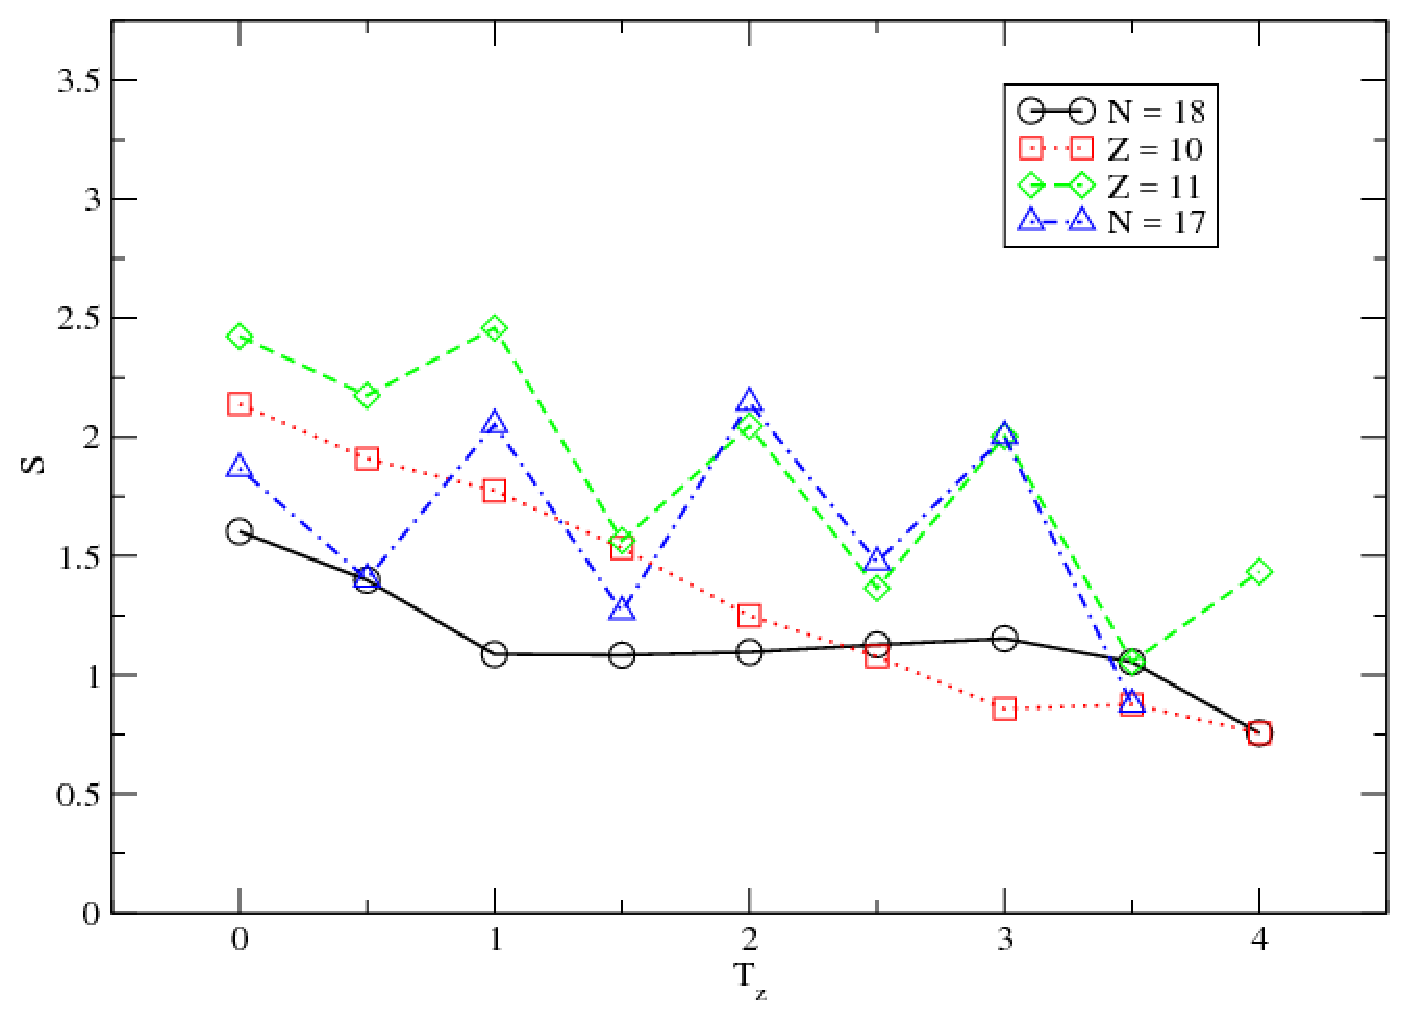
\includegraphics[width=.75\textwidth,clip]{Figures/s_vs_tz_sd}
        \caption{Entanglement entropy versus isospin for particle-hole conjugate nuclei in the
\textit{sd}-shell. Entanglement entropy tends to continuously decrease for even-even and even-odd 
numbers of protons and neutrons (see even-Z isotopes and even-N isotones), but 
to jump up for odd-odd nuclei (see odd-Z isotopes
and odd-N isotones).}
    \label{fig: tz1}
\end{figure}




\subsection{Dialing the Strength of the Proton-Neutron Interaction}

The shell-model code BIGSTICK to allows for scaling of the proton-neutron 
interaction term when working in the explicit proton-neutron 
formalism. Thus the two-body part of Hamiltonian is of the form
\begin{equation}
    H = H_{pp} + H_{nn} + \lambda H_{pn}.
\end{equation}
In BIGSTICK, this means scaling the two-body interaction
matrix elements by $\lambda$:
\begin{equation}
    \lambda\bra{ab}V^{(pn)}\ket{cd}
\end{equation}
We examined the relationship between the strength of the 
proton-neutron interaction and the relative proton-neutron 
entanglement entropy for the ground state of a number of 
nuclei. (See Figure \ref{fig: l28ne}.)
The scaling factor $\lambda$ was varied from zero, i.e.
no proton-neutron interaction at all, to an order of magnitude
above unity. A scaling factor of $\lambda=1$ is a fully realistic 
calculation.
The entanglement 
entropy will be zero when $\lambda$ is zero because in this
case there is no interaction between protons and neutrons. 
Essentially we have two separate and non-interacting 
model spaces. The entanglement entropy will increase as
the strength of the interaction increases. 

If our hypothesis that $N>Z$ nuclei converge faster in the 
proton-neutron formalism than $N=Z$ nuclei is correct, then 
we might expect different behavior in the
$S$ vs $\lambda$ curves for $N>Z$ and $N=Z$ nuclei.
In fact what we find is that the $S$ vs $\lambda$
curve for $N>Z$ nuclei falls below the one for $N=Z$ 
nuclei for nuclei of the same model space dimension.
Having the same model space dimension means that
the two nuclei will also have the same maximum 
proton-neutron entanglement entropy.
This is accomplished by comparing nuclei which are
particle-hole conjugates.

\begin{figure}[t]
    \centering
    \includegraphics[width=.75\textwidth,clip]{Figures/s_vs_lambda_28ne}
    \caption{Proton-neutron entanglement entropy as a function of the proton-neutron
two-body interaction matrix element scaling factor \boldmath$\lambda$. Entanglement entropy
is necessarily zero when $\lambda=0$. $\lambda<0$ value are non-physical but
shed light on the behavior of the coupling. $^{28}$Ne, with an unequal number 
of protons and neutrons, has the lowest entanglement entropy for values of 
$\lambda>0$ up until about seven times the realistic value of $\lambda=1$.}
    \label{fig: l28ne}
\end{figure}

Figure \ref{fig: l28ne} shows the dramatic difference between the 
$S$ versus $\lambda$ curves of nuclei with $N=Z$ versus $N>Z$.
$N>Z$ have significantly lower proton-neutron entanglement entropy
for values of $\lambda$ greater than zero up to about five to
seven times the realistic scaling of the proton-neutron
interaction. 


\section{Modified Nuclear Interactions}
We have shown that proton-neutron entanglement entropy is inversely correlated with
isospin; however it is not obvious why this is the case. 
In this section I summarize some of the attempts made to 
isolate the physics responsible for the behavior demonstrated 
in the previous chapter. To this end,
I recomputed the entanglement entropy versus proton-neutron interaction
strength (via the scaling factor $\lambda$) for several different
nucleon-nucleon interactions.

The first series of calculations were made with \textit{zero single particle energies}.
In this interaction we start with the fully realistic nuclear
interaction and then set the single particle energies equal 
to zero. In the many-body Hamiltonian,
\begin{equation}
    H = \sum_{ij} \epsilon_{ij}a^\dagger_ia_i + \sum_{ijkl} a^\dagger_ia^\dagger_jV_{ijkl}a_ka_l
\end{equation}
the single particle energies are $\epsilon_{ij}$.

The second series of calculations were made with \textit{traceless interactions} (see Figure \ref{fignmp}).
In this interaction we again start with the fully realistic nuclear
interaction and then remove the monopole terms in the two-body 
interaction. These are terms of the form\cite{Caurier}
\begin{equation}
    V_{mono} = \sum_{ab} \hat{n}_a(\hat{n}_b-\delta_{ab})U(ab),
\end{equation}
where $\hat{n}$ are number operators. These are related to shell structure.

The third series of calculations were made with only an attractive
quadrupole-quadrupole interaction\cite{Schuck} (see Figure \ref{figqq}). This interaction is derived from
the nuclear quadrupole moment\cite{Wong,Schuck},
\begin{equation}
    Q_{ij}=\int \rho(\vec{r})(3x_ix_j-r^2\delta_{id})d\vec{r},
\end{equation}
a tensor operator for which for microscopic expectation value for a system
of nuclear matter is given by\cite{Heyde,Schuck}
\begin{equation}
    Q_\alpha(J,M) = \bra{\psi_{JM}(r_i)}\sum_i(3x^\alpha_i-r_i^2)\ket{\psi_{JM}(r_i)},
\end{equation}
where $\alpha$ is the directional orientation of the quadrupole moment of 
interest.

The fourth series of calculations were made with an attractive pairing interaction (see Figure \ref{figpair}).
A problem arose when computing entanglement entropies for this interaction.
The pairing interaction is known to be highly degenerate, and in cases where the eigenstates are
nearly degenerate, the Lanczos method performs poorly. 
This is because the Lanczos method is susceptible to loss
of orthogonality of eigenstates due to numerical noise.
In order to counteract this, the two-body interaction
matrix elements were slightly modified. A very small random
interaction was added to the matrix elements in order to
desensitize the Lanczos algorithm to the degeneracies.
\begin{figure}[h]
    \centering

        \includegraphics[width=.75\textwidth,clip]{Figures/s_vs_lambda_nmp_ne}
        \caption{Entanglement entropy with a traceless interaction.}
        \label{fignmp}
\end{figure}
\begin{figure}
        \centering
        \includegraphics[width=.75\textwidth,clip]{Figures/s_vs_lambda_qq_ne}
        \caption{Entanglement entropy with an attractive quadrupole-quadrupole interaction.}
        \label{figqq}
\end{figure}

\begin{figure}
    \centering
    \includegraphics[width=.75\textwidth,clip]{Figures/s_vs_lambda_pair_ne}
    \caption{Attractive pairing interaction: Ne and PH-Conjugates.}
    \label{figpair}
\end{figure}

We also ran several trials with particle-hole conjugate nuclei 
with random two-body interactions (see Figure \ref{figrand1} and Figure \ref{figrand2}). This means that all of the
physics is removed and all that remains are properties of the 
model space. Because any given random interaction may not be particularly 
enlightening, we ran up to 1000 calculations with unique random
interactions and plotted a histogram of the ground state
entanglement entropy. In these calculations we lose the 
correlation between isospin and proton-neutron entanglement 
entropy. We often see normal distributions of the entanglement
entropy for a given nucleus, and two unique modes for the 
distributions within a particle-hole conjugate triplet.

\begin{figure}
    \centering
    \includegraphics[width=.75\textwidth,clip]{Figures/rand_s_ne}
    \caption{Random interactions exhibiting a bimodal distribution of entanglement entropy. No apparent
correlation between entanglement entropy and ratio of protons to neutrons.}
    \label{figrand1}
\end{figure}

\begin{figure}
    \centering
    \includegraphics[width=.75\textwidth,clip]{Figures/rand_s_ne_nmp}
    \caption{Random traceless interactions exhibiting a unimodal distribution of entanglement entropy. No
apparent correlation between entanglement entropy and ration of protons to neutrons. $N=Z$ nuclei have the
same entanglement entropy for all interactions, as expected.}
    \label{figrand2}
\end{figure}

This study failed to reveal the source of the isospin dependence of the
proton-neutron entanglement entropy. The phenomenon is not unique to
any of: the pairing interaction, the quadrapole-quadrapole interaction,
the full interaction with or without the monopole terms.

\section{Toy Model}

I constructed a toy model to investigate the behavior of 
entanglement entropy of coupled systems, in an attempt 
to better understand the behavior seen in real nuclei such as in Figure 
\ref{fig: l28ne}. In the toy model, I consider a subspace A and a subspace B, 
which together form a 
bipartite system $\mathcal{H}_{AB}=\mathcal{H}_A\otimes\mathcal{H}_B$.
$\mathcal{H}_{AB}$ is spanned by a coupled basis:
\begin{equation}
    \ket{i} = \ket{a}\ket{b} = \ket{a}\otimes \ket{b},
\end{equation}
where $\ket{a}$ are the basis states of $\mathcal{H}_A$ and 
$\ket{b}$ are the basis states of $\mathcal{H}_B$. A Hamiltonian operator of this
bipartite space could be written as
\begin{equation}
    \hat{H} = \hat{H}_A + \hat{H}_B + \hat{H}_{AB} 
\end{equation}
where $\hat{H}_A =\hat{h}_a \otimes \hat{1}$ is an operator which acts purely in the A space,
$\hat{H}_B=\hat{1}\otimes\hat{h}_b$ is an operator which acts purely in the B space and
$\hat{H}_{AB}=\hat{V}\otimes\hat{W}$ is an operator which acts on both spaces. 
We are interested in the behavior of the system as a function of the strength of the
coupling term $\hat{H}_{AB}$. I assume for convenience that we have already diagonalized $\hat{H}_A$
and $\hat{H}_B$. I choose single particle spaces with constant energy
spacing:
\begin{equation}
	E_a \equiv \hat{h}_A \ket{a} = a \epsilon 
\end{equation}
for $a=1,..,N$ and $\epsilon = const.$, and similarly for $\hat{H}_B$.

For $\hat{H}_{AB}$ I choose an operator which is the tensor product of an 
operator $\hat{V}$ in $\mathcal{H}_A$ and an operator $\hat{W}$ in $\mathcal{H}_B$. I am only interested in
the behavior of the system as a function of the strength of the interaction between
the subsystems, so the exact structure of each subsystem is not important. Therefore, 
I simply choose to fill these two matrices with a random Gaussian number generator. I 
symmetrically fill an $N\times N$ matrix with random numbers centered at zero with a
standard deviation of $2\sigma$ for the diagonal matrix elements, 
and $\sigma$ for the off-diagonal matrix, a standard practice for generating 
real, symmetric random matrices. Finally, I include a two-body matrix elements 
(TBME) scaling factor $\lambda$:
\begin{equation}
	\hat{H}_{AB} = \lambda\hat{V}\otimes \hat{W}
\end{equation}
It is now straightforward to calculate the matrix elements of the Hamiltonian.
As above, let $a$, $a'$ label the proton states and $b$, $b'$ 
label the neutron states. These run from 1 to $N$. Now let $i = a + N(b-1)$ label 
the many-body state, which runs from 1 to $N^2$. Then
\begin{equation}\label{eq:1}
	\bra{i'}\hat{H}\ket{i} =     
	H_{i',i} = \delta_{a'a}\delta_{b'b}(E_a+E_b)+\lambda V_{a'a} W_{b'b}.
\end{equation}
$V_{a'a}$ and $W_{b'b}$ are real, symmetric, $N \times N$ 
random matrices with Gaussian distributions:
\begin{equation}
    P(V_{aa'}) \sim exp\Big(-\frac{V_{aa'}^2}{2\sigma^2(1+\delta_{a'a})}\Big),
\end{equation}
a Gaussian distribution of $\sigma$ for the off-diagonals and $2\sigma$ for the diagonals.

Once we diagonalize the model Hamiltonian, we want to quantify
how the entanglement entropy is affected by the coupling-
term scaling factor $\lambda$ and by the two interactions
are the same $W=V$ or different $W\neq V$. This is meant to
model the behavior of the nuclear Hamiltonian when and its
distinct $S_{pn}$ versus $\lambda$ curves for when
the number of protons is the same or different from 
the number of neutrons. 

Suppose that we diagonalize the Hamiltonian and that
\begin{equation}
\hat{H} \ket{\psi}_i = E_i \ket{\psi}_i
\end{equation}
defines our $N^2$ eigenstates. Any given state can be written as 
\begin{equation}
\ket{\psi} = \sum_i c_i \ket{i} = \sum_{a,b} c_{ab} \ket{a}\ket{b},
\end{equation}
and so the reduced density matrix $\rho_A$  of $\ket{\Psi}$ is the partial trace, 
\begin{equation}
    \rho_A = tr_a\ \rho.
\end{equation}
Given our choice of indexing, this is computed as
\begin{equation}
    \rho_p(a',a) = \sum_{b=1}^N c_{a'b}c_{ab}^*.
\end{equation}
We can now define the proton-neutron entanglement 
entropy of the state described by $\rho$ to be the 
\textit{von Neumann} entropy of the reduced density 
matrix $\rho_p$,
\begin{equation}
    S_{pn} = -tr \rho_p\ \ln \rho_p.
\end{equation}
If we first diagonalize $\rho_p$ to find its $N$ eigenvalues 
$\gamma_i^2$ then the entanglement entropy becomes
\begin{equation}
    S_{pn} = - \sum_{i=1}^N \gamma_i^2\ \ln \gamma_i^2.
\end{equation}
This quantity measures the entanglement entropy, or 
the mixing of quantum bits, of the two subspaces in a 
given state of the Hamiltonian.

In the first adaption of this toy model we has Hamiltonian matrix elements
exactly as they appear in equation (\ref{eq:1}).
Here, $\epsilon=1$, $\sigma=1$, and 
two curves are plotted: one in which the random matrices 
$V$ and $W$ are the same and one in which they are different. 
In these models we saw that when the two interactions $W$ and $V$ are the same, the 
entanglement entropy tends towards some finite non-zero value, 
whereas when $W$ and $V$ are different, the 
entanglement entropy falls off to zero. This tells us that the entanglement 
entropy can differ between two systems of the same dimension depending on 
the similarity of the interactions acting between the subspaces. Mathematically this has to do with the 
orthogonality of the eigenstates of the interactions within each subspace.
In another adaption of the model, we start 
with two identical subspaces and then slowly change 
one of the subspaces to be different from the original. 
\begin{equation}\label{modeld}
	H = E^V + E^W + \lambda(V\otimes(V+\delta W))
\end{equation}
In doing so we can see in Figure \ref{opt3} that as the two interactions diverge, 
the entanglement entropy of the system falls off from its
maximum convergent value. 
When the perturbative parameter $\delta=0$, equation (\ref{modeld})
reduces to equation (\ref{eq:1}) for the case when $W=V$.

\begin{figure}
    \centering
    \includegraphics[width=	.75\textwidth,clip]{Figures/toymodel1delta}
    \caption{Toy Model with perturbative variance of the interaction $W$ away from $V$. 
    The subspaces containing the $V$ interaction has the same dimensions as the 
    subspace containing the $W$ interaction. See equation (\ref{modeld}).}
    \label{opt3}
\end{figure}

In an attempt to get convergence to non-zero entanglement entropies
when $W\neq V$, which is what we see in the nuclear calculations, I suggested 
the following Hamiltonian on the grounds that a constant term may 
prevent the entanglement entropy from converging to zero when the 
two species of interactions are different:
\begin{equation}
    H_{i',i} = \delta_{a'a}\delta_{b'b}(E_a+E_b)+\lambda
\big( V_{a'a} W_{b'b} + V_{a'a} + W_{b'b} \big ),
\end{equation}
which implicitly is a Hamiltonian of the form
\begin{equation}
    H = E^V + E^W + \lambda ( V\otimes W + V\otimes I + I \otimes W ),
\end{equation}
where $E$ is diagonal. By using an explicitly non-separable interaction,
we obtained the desirable feature than $W\neq V$ curves converged to
non-zero entanglement entropy. However, curves generated with different
random number generator seeds produced varying results, some exhibiting
anomalous spikes in entropy near the origin. 

The next most obvious 
adaption was to simply include a several terms in the coupling part of the Hamiltonian:
\begin{equation}
    H_{i',i} = \delta_{a'a}\delta_{b'b}(E_a+E_b)+\lambda\big( 
\sum_i V_{a'a}^i W_{b'b}^i  \big ),
\end{equation}
which is a Hamiltonian of the form:
\begin{equation}
    H = E^{(V)} + E^{(W)} + \lambda (\sum_i V_i \otimes W_i ),
\end{equation}
where each 
The results of this toy model are shown in Figure \ref{best}.
This version of the toy model has the following 
features: 
\begin{itemize}[noitemsep]
\item Entanglement entropy goes to zero at the origin
\item Dependence on the random number generator seed goes down
    with the number of terms in the sum
\item Entanglement entropy convergences to nonzero entanglement 
    entropies at large $\lambda$ for different 
subspaces, and 
\item Very few anomalous features, such as spikes in entanglement entropy
\end{itemize}

However, the model still doesn't have the same features as the
realistic proton-neutron entanglement entropy, namely, symmetric
entanglement entropy curves when the both species' interactions
are identical, and, when the interactions are different: lower entanglement entropy 
for positive $\lambda$ and higher entanglement entropy for negative $\lambda$.
See Figure \ref{best} (a) and (b) for comparison.
Several dozen other toy model Hamiltonians were investigated, including those with different 
single species interactions, and models with different dimensions. However, I
 failed to find a model which reliably produces $S$ versus $\lambda$ curves with 
the same topology as in the nuclear Hamiltonian.
\begin{figure}[t]
    \centering
	\subfigure[]{
		\includegraphics[width=.75\textwidth,clip]{Figures/toymodel3}
	}
	\qquad
	\subfigure[]{
		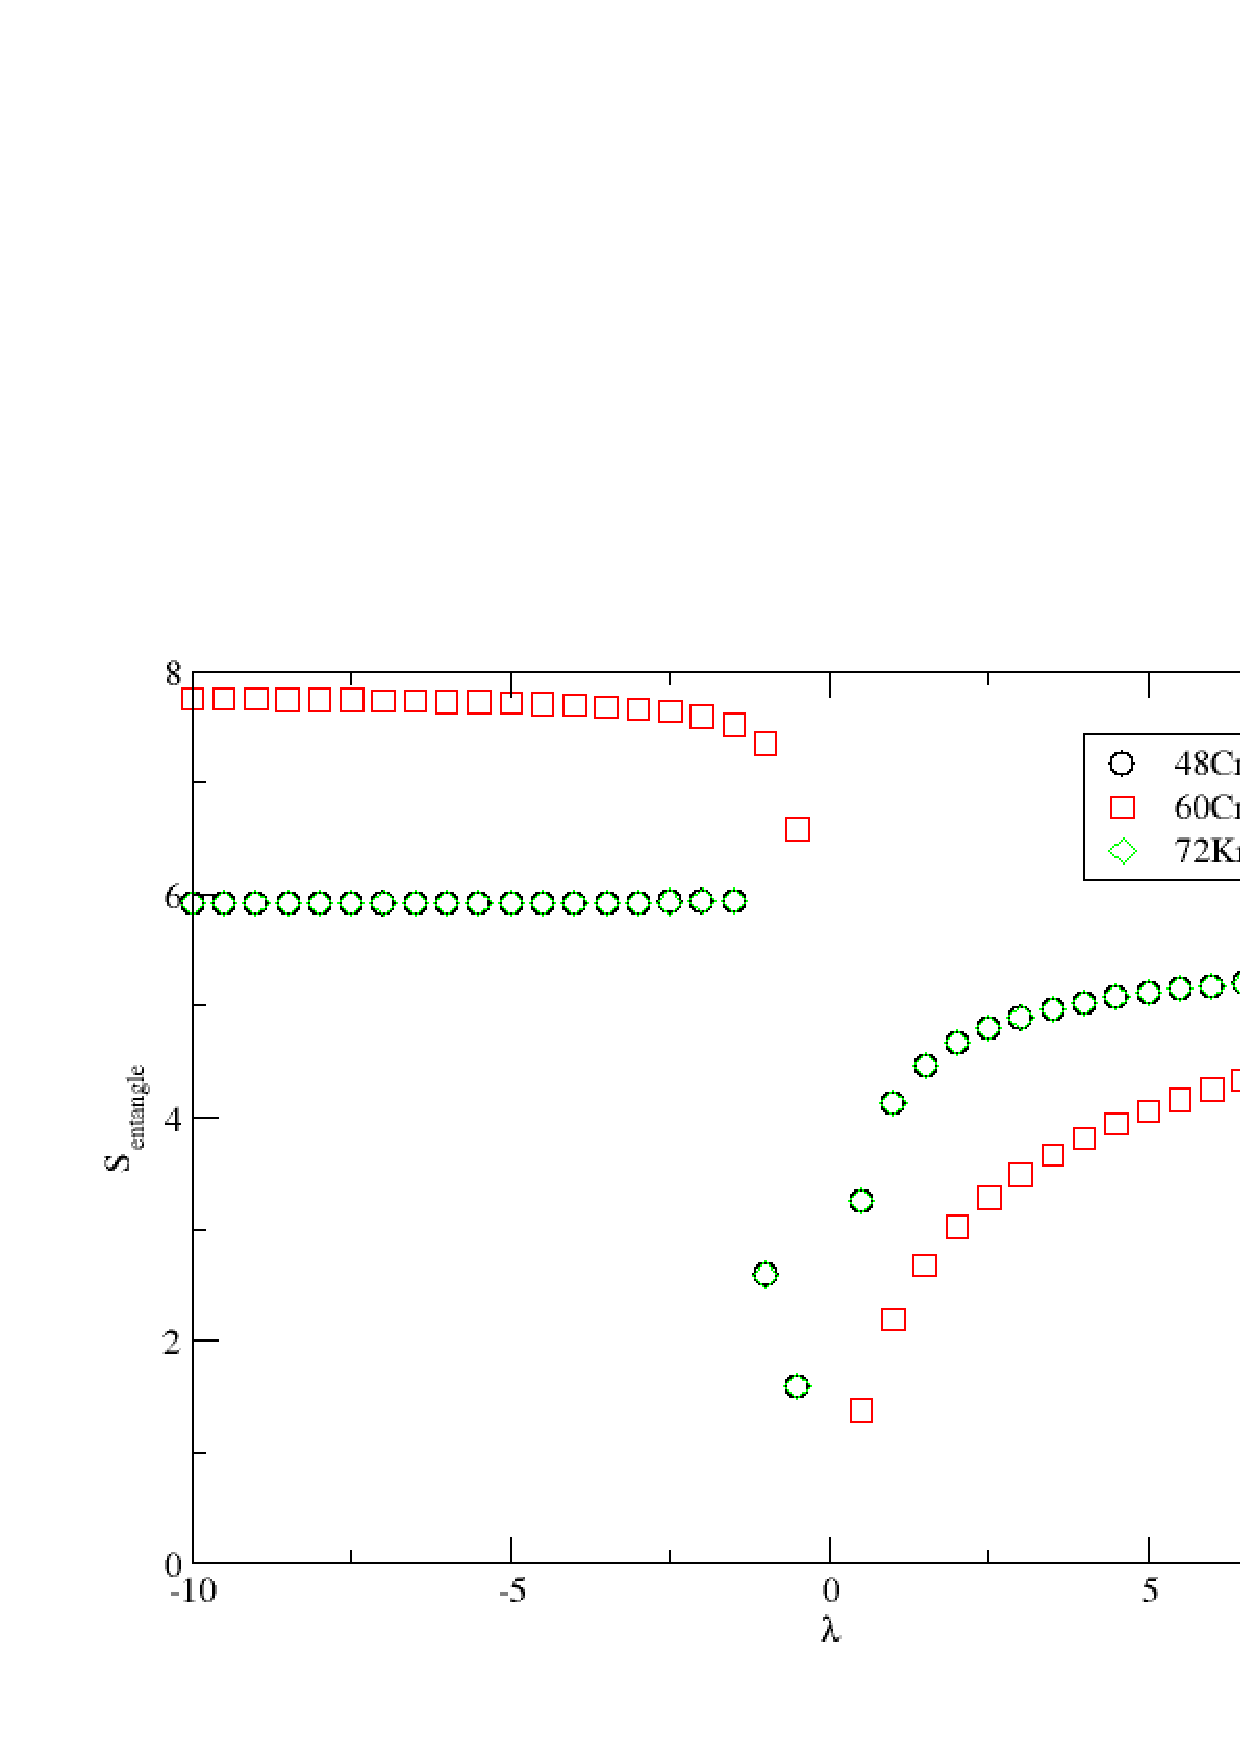
\includegraphics[width=	.85\textwidth,clip]{Figures/s_vs_lambda_48crnmp}
	}
	\caption{Entanglement entropy $S$ versus scaling factor $\lambda$ for (a) toy model 
    with non-separable two-body terms, and (b) nuclei in the \textit{pf}-shell with a traceless interaction.}   
	\label{best}
\end{figure}


\section{Summary on Entanglement Entropy}
We investigated the properties of the proton-neutron entanglement entropy,
which is an indicator used to determine whether or not certain wavefunctions
could be represented more efficiently in some basis. We showed that nuclei with
unequal numbers of protons and neutrons have a lower entanglement entropy, which
means that $N>Z$ nuclei may have even more efficient representations. We
attempted to understand the properties of the entanglement entropy, but more 
investigation is needed. The toy model we investigated tells us that the phenomenon
of higher entanglement entropy in systems with identical subspaces is more
ubiquitous than the nuclear many-body problem. Moving on from this section,
readers should keep in mind that we have evidence for the existence of 
efficient representations of our nuclear wavefunctions, but have yet to 
inquire about which basis will yield these efficient representations. This will
be addressed in the next chapter.







\chapter{PROTON-NEUTRON DECOMPOSITION}
\label{chap:decomp}

In the previous chapter, we studied the distribution of wavefunction coefficients
in order to provide evidence that there exists a basis in which our nuclear
wavefunctions could be truncated, thus allowing more efficient representation
of the wavefunctions. Ultimately our goal is to find a basis in which our 
Hamiltonian can be truncated.
In this chapter I will examine a decomposition of wavefunctions which
corresponds to a particular framework for computing truncated Hamiltonian matrix
elements.

We will be assuming that our Hamiltonian can be decomposed as
\begin{equation}\label{htotal}
	\hat{H} = \hat{H}_{proton} + \hat{H}_{neutron} + \hat{H}_{proton-neutron}
\end{equation}
where $\hat{H}_{proton}$ contains all interactions between protons, 
$\hat{H}_{neutron}$ contains all interactions between neutrons, and $\hat{H}_{proton-neutron}$ contains
all remaining interactions between protons and neutrons. Then we call the 
eigenstates of the pure-proton Hamiltonian $\ket{\pi}$, as in
\begin{equation}\label{hppp}
	H_{proton}\ket{\pi} = E_p\ket{\pi},
\end{equation}
and the eigenstates of the pure-neutron Hamiltonian are equivalently
define for $\hat{H}_{neutron}$ and $\ket{\nu}$. 
Roughly speaking, our proposed truncation 
scheme is to compute the full Hamiltonian (\ref{htotal}) in a basis
built up from the coupled eigenstates of $\hat{H}_{proton}$ and $\hat{H}_{neutron}$.
It was therefore worth decomposing existing wavefunctions $\ket{\Psi}$
into the eigenstates of both pure-proton interaction operators and 
pure-neutron interaction operators. This will tell us how whether or not
truncating a basis of coupled pure-proton and pure-neutron wavefunctions
will be viable. To see why, consider an arbitrary wavefunction $\ket{\Psi}$.
To expand $\ket{\Psi}$ into a basis $\{\ket{\alpha}\}$, one first computes the
coefficients
\begin{equation}
    c_\alpha = \braket{\alpha}{\Psi}.
\end{equation}
If some significant subset of the coefficients $\{\ket{\alpha}\}$ are much smaller than the rest,
then the full wavefunction,
\begin{equation}
    \ket{\Psi} = \sum_\alpha c_\alpha \ket{\alpha},
\end{equation}
could be represented by just a few terms. What we care about is the magnitude of
the coefficients $\{\ket{\alpha}\}$, thus we could instead compute
\begin{equation}\label{coef2}
    |c_\alpha|^2 = \braket{\Psi}{\alpha}\braket{\alpha}{\Psi},
\end{equation}
where the object $\ket{\alpha}\bra{\alpha}$ is a projection operator.

We computed the equivalent set of coefficients (\ref{coef2}) for our
nuclear wavefunctions projected onto the eigenstates of $\hat{H}_{proton}$ and
$\hat{H}_{neutron}$.
This was done using existing
capabilities in BIGSTICK to compute transition strength functions. In particular I
used the option to decompose wavefunctions onto scalar operators\cite{Johnson18}.
To do this, we first solve for the wavefunction $\ket{\Psi}$ for some nucleus.
Then BIGSTICK solves equation (\ref{hppp}) and the equivalent equation for the
neutron Hamiltonian, using its Lanczos capabilities to find low-lying 
eigenstates $\ket{\pi_a}$ (or $\ket{\nu_a}$). Then, the nuclear wavefunction is projected
onto these eigenstates in the following manner:
\begin{equation}\begin{split}
	\braket{\pi_a}{\Psi} &= \bra{\pi_a}\sum_{a,b}\tilde{\Psi}_{ab}\ket{\pi_a}\ket{\nu_b} \\
		              &= \sum_{b}\tilde{\Psi}_{ab}\ket{\nu_b}.
\end{split}\end{equation}
The strengths of these projections is then computed as
\begin{equation}\begin{split}
        \braket{\Psi}{\pi_a'}\braket{\pi_a}{\Psi} &= \sum_b \tilde{\Psi}^*_{a'b}\tilde{\Psi}_{ab} \\
 		&= \sum_b^{N_{keep}} |\Psi_{ab}|^2\\
        & \equiv c_a^2.
\end{split}\end{equation}
The quantities $c_a^2$ are the strengths of the projection of a wavefunction $\ket{\Psi}$
onto the proton-proton interaction eigenstate $\ket{\pi_a}$. Since we are assuming a set of normalized 
wavefunctions in our basis, 
\begin{equation}
1 = \sum_a \braket{\pi_a}{\pi_a},
\end{equation}
and thus the strengths $c_a^2$ are the fractions of the total wavefuntion $\ket{\Psi}$
contained in the state $\ket{\pi_a}$.

I projected nuclear wavefunctions onto the eigenstates of the proton Hamiltonian
of the neutron Hamiltonian and plotted the strengths $c_X^2$ for each interaction
as a function of the eigenstate number. A typical set of results in shown in
Figure \ref{fig: pndecomp1} and Figure \ref{fig: pndecomp2}.
The vertical axis is the strength of the decomposition onto the eigenstate
of either the proton Hamiltonian or the
neutron Hamiltonian with the $X^{th}$ lowest energy. Each plots has two sets
of values, one for each of two particle-hole conjugate nuclei in the \textit{sd}-shell:
one being the proton (PP) decomposition and the other being the neutron (NN) decomposition.

There are two important conclusions to be drawn from these decompositions. The first is that the strengths
fall off rapidly in the first handful of states. This suggests than
a truncation of the coupled pure-proton and pure-neutron eigenstates could a viable 
method for obtaining approximate wavefunctions. However it is already known that 
this is the case for light nuclei\cite{Papenbrock03,Papenbrock04,Papenbrock05}. The second
important feature is apparent when plotting the strength function
decompositions for particle-hole conjugate nuclei on the same plot. We find that
even though these pairs of nuclei have the same dimensions in their shell model spaces,
nuclei for which $N>Z$ have strengths which are significantly lower than their 
$N=Z$ conjugates. This is further evidence that the same proposed truncation scheme
may be even more effective in heavier nuclei where $N>Z$.

\begin{figure}
    \centering
    \includegraphics[width=4.5in]{Figures/decomp_na}
    \caption{Strength decomposition of nuclear wavefunctions into eigenstates of
    the proton-proton or neutron-neutron interaction for two particle-hole conjugate
    nuclei in the \textit{sd}-shell. Strengths fall off exponentially. } 
    \label{fig: pndecomp1}
\end{figure}

\begin{figure}
    \centering
    \includegraphics[width=4.5in]{Figures/decomp_na_ln}
    \caption{Strength decomposition of nuclear wavefunctions into eigenstates of
    the proton-proton or neutron-neutron interaction for two particle-hole conjugate
    nuclei in the \textit{sd}-shell. The decomposition strengths of $^{28}$Na, with an unequal number of protons
    and neutrons, fall off faster than its conjugate, suggesting that fewer states
    are necessary to represent it. } 
    \label{fig: pndecomp2}
\end{figure}

\chapter{PNISM}
\label{chap:PNISM}

% By labeling the chapter, I can refer to it later using the
% label. (\ref{chap:intro}, \pageref{chap:intro}) Latex will take care
% of the numbering.
Finally, we turn to the main subject of this thesis, our Proton-Neutron Interacting
Shell Model (PNISM) code. We are motivated by the results of the previous chapters; 
it is known that SVD eigenvalues of wavefunction coefficients fall off exponentially,
and we have seen that they fall off even faster in nuclei with unequal numbers
of protons and neutrons. We also argued that the basis states formed from
the eigenstates of the proton interaction and the neutron interaction could likely
allow for truncated wavefunctions. We have reason to believe that truncation of 
the model space in a weakly coupled proton-neutron basis might be an especially effective
approximation for heavier nuclei with more neutrons than protons. 
We set out to write a code that couples together eigenstates of the proton Hamiltonian and 
eigenstates of the neutron Hamiltonian to create a many-proton many-neutron basis.
The matrix elements of the full Hamiltonian are then computed in this basis, which is
truncated.

This chapter will derive the equations used to carry out the calculation of the
Hamiltonian matrix elements from the eigenstates computed by the interacting 
shell model code BIGSTICK. Calculation of the one-body density matrices of the
resulting wavefunctions is also discussed. The following chapter will discuss
the details of the code itself.

\section{The Hamiltonian}
We write the nuclear Hamiltonian in explicit proton-neutron formalism. The 
Hamiltonian operator in the second quantization formalism,
\begin{equation}
	\hat{H}=\sum_{ab}\bra{a}T\ket{b}\hat{c}^\dagger_a\hat{c}_b
    +\frac{1}{4}\sum_{abcd}\bra{ab}V\ket{cd}\hat{c}^\dagger_a\hat{c}^\dagger_b\hat{c}_c\hat{c}_d,
\end{equation}
can be written as a sum of terms separated by nucleon species\cite{Johnson13}:
\begin{equation}\label{sep}
    \hat{H} = \hat{H}_p + \hat{H}_n + \hat{H}_{pp} + \hat{H}_{nn} + \hat{H}_{pn},
\end{equation}
where $\hat{H}_p$ and $\hat{H}_{pp}$ are one- and two-body Hamiltonians, respectively, which act
only on protons, $\hat{H}_n$ and $\hat{H}_{nn}$ act only on neutrons, and $\hat{H}_{pn}$
contains the remaining interactions between proton and neutrons. 
To this end, it is useful to define the two body creation operator\cite{Schuck}:
\begin{equation}
    \hat{A}_{JM}^\dagger(ab)\equiv [c_a^\dagger \otimes c_b ^\dagger]_{JM}
\end{equation}
Here, the total angular momentum $J$ and the azimuthal or magnetic quantum number 
$M=J_z$ are needed for the coupling of the two one-body creation operators, 
via Clebsch-Gordan coefficients\cite{Edmonds}:
\begin{equation}
    [c_a^\dagger \otimes c_b ^\dagger]_{JM} = 
        \sum_{m_am_b} (j_am_a, j_bm_b|JM)\hat{c}^\dagger_{j_am_a}
        \hat{c}^\dagger_{j_bm_b}.
\end{equation}
The two-body creation and annihilation operators\cite{Feshbach} with fixed $J$ and $M$ are thus, respectively:
\begin{equation}\begin{split}\label{pairs}
    & A^\dagger_{JM} = \sum_{m_am_b} (j_a m_a, j_b m_b | JM ) c^\dagger_{j_am_a} 
c^\dagger_{j_bm_b}, \textrm{ and} \\
    & A_{JM} = \sum_{m_cm_d} (j_c m_c, j_d m_d | JM ) c_{j_cm_c} c_{j_dm_d}.
\end{split}\end{equation}
These will be used later in the derivation of the proton-neutron interaction
matrix elements.
With these definitions, two-body states with proper normalization are\cite{Brussard}
\begin{equation}
    \ket{ab; JM} \equiv \frac{1}{\sqrt{1+\delta_{ab}}}
       \hat{A}^\dagger_{JM}(ab)\ket{0}.
\end{equation}
The two-body part of the Hamiltonian is thus expressed
\begin{equation}\begin{split}
    \hat{H_{2b}} &= \sum_{abcd}{c}^\dagger_a{c}^\dagger_b\bra{ab}V\ket{cd}
        \hat{c}_c\hat{c}_d \\
    &= \frac{1}{4}\sum_{abcd}\zeta_{ab}\zeta_{cd}
    \sum_{J}\bra{ab;JM}V\ket{cd;JM}\sum_{M}{A}^\dagger_{JM}(ab){A}_{JM}(cd)
\end{split}\end{equation}
where $\zeta_{ab}\equiv\sqrt{(1+\delta_{ab})}$.
Our next move is to change to an explicit proton-neutron decomposition.
This can be done by using the states $\frac{1}{\sqrt{2}}
(\ket{\pi\nu}-\ket{\nu\pi})$, $\frac{1}{2}(\ket{\pi\nu}+\ket{\nu\pi})$,$\ket{\pi\pi}
$, and $\ket{\nu\nu}$ to isolate operators by the nucleon species on which they act. 
The result is the following proton-proton two-body interaction:
\begin{equation}\begin{split}
    \hat{H}_{pp} =
    \frac{1}{4}\sum_{abcd}\zeta_{ab}\zeta_{cd}
    \sum_{J}V_{J}^{pp}(ab,cd)\sum_{M}\hat{A}^\dagger_{JM}(a_\pi b_\pi)\hat{A}_{JM}(c_\pi d_\pi).
\end{split}\end{equation}
$\hat{H}_{nn}$ has the same form. We will not use these directly but it is 
useful to see how the interaction is separated. The proton-neutron interaction is
the only term that will be used directly in our code:
\begin{equation} \label{eqn: hpn}
    H_{pn} = \sum_{abcd}\sum_J V_J^{(pn)}(ab,cd) 
\sum_M A_{JM}^\dagger(a_\pi b_\nu) A_{JM}(c_\pi d_\nu).
\end{equation}


\section{The Basis}
We have a Hamiltonian of the form (\ref{sep}) and in order to compute its matrix
elements, we need to choose a basis, one which we hope we can truncate effectively. In this
section I will explain our choice of basis and how we select which states to truncate.
In the future we will want to develop a more sophisticated approximation scheme to 
improve our results. 
For now we first solve
\begin{equation}\begin{split}\label{ppnnsol}
    (\hat{H}_p + \hat{H}_{pp})\ket{\Psi_p}&= E_p\ket{\Psi_p} \textrm{ and}\\
    (\hat{H}_n+H_{nn})\ket{\Psi_n}&=E_n\ket{\Psi_n},
\end{split}\end{equation}
and set our uncoupled basis states equal to the solutions:
\begin{equation}\begin{split}\label{plusminus}
    \ket{J_p^{\pi_p},\alpha_p}&=\ket{\Psi_p},\\
    \ket{J_n^{\pi_n},\beta_n}&=\ket{\Psi_n},
\end{split}\end{equation}
where $J_p$ is the total angular momentum of the proton state, $\pi_p$ is its parity,
and $\alpha_p$ is just a state label, and equivalently for the neutron states. 
We build our many-body basis states by coupling together these proton and
neutron states: 
\begin{equation}\label{cbasis}
	\ket{J_p^{\pi_p},\alpha_p}\otimes\ket{J_n^{\pi_n},\beta_n}.
\end{equation}

Our
solutions to (\ref{ppnnsol}) yield $d_\pi$ pure proton eigenstates and $d_\pi$ pure
neutron eigenstates. The eigenstates of a Hermitian operator form a complete set 
of orthogonal eigenvectors. Assuming these are normalized, any many-body 
wavefunction can be expanded:
\begin{equation}
    \ket{\Psi} = \sum_{\alpha_p}^{d_\pi}\sum_{\beta_n}^{d_\nu}\Psi_{\alpha_p\beta_n} \ket{J_p^{\pi_p},\alpha_p}\otimes\ket{J_n^{\pi_n},\beta_n}.
\end{equation}
Therefore these states can be used to compute the matrix elements of the full Hamiltonian
(\ref{sep}), where $\hat{H}_p + \hat{H}_{pp}$ and $\hat{H}_n+H_{nn}$ are now
used in their diagonal forms.

So far all we have done is to solve the nuclear Hamiltonian in a basis of
coupled proton and neutron states by solving the proton and neutron 
interactions separately. The computational advantage to this
procedure lies in the prospect of truncating the model space. In doing so, we 
will have to make choices to ensure that the eigenstates of the truncated
Hamiltonian remain eigenstates of $J^2$. 
If we were to truncate the basis in an M-Scheme procedure, then our
solutions would not be guaranteed to have good total angular momentum. To see why,
consider the following example for a two state system. Imagine a basis with two
states $\frac{1}{\sqrt{2}}(\ket{z;+}+\ket{z;-})$ and
$\frac{1}{\sqrt{2}}(\ket{z;+}-\ket{z;-})$. If we were
truncate to just one of either of these states, then any solution in the truncated
basis could not be an eigenstate of $\hat{S}_z$. Similarly, a truncated M-scheme
basis is not guaranteed to have good total angular momentum. Therefore,
we choose a basis with good total angular momentum so that even once we
truncate the basis we are guaranteed to get solutions with good total angular momentum.
This is called a J-scheme.

Therefore we choose to couple our proton and neutron states in such a way as to
be eigenstates of $\hat{J}^2$:
\begin{equation}\label{cbasisJ}
	[\ket{J_p^{\pi_p},\alpha_p}\otimes\ket{J_n^{\pi_n},\beta_n}]_{J^\pi}\equiv
	\ket{J_p^{\pi_p},\alpha_p,J_n^{\pi_n},\beta_n;J^\pi},
\end{equation}
A wavefunction expanded in this basis is of the form
\begin{equation}
    \ket{\Psi} = \sum_{\alpha_p\beta_n}^{Q}\Psi_{\alpha_p\beta_n} 
    \ket{J_p^{\pi_p},\alpha_p,J_n^{\pi_n},\beta_n;J^\pi},
\end{equation}
and is guaranteed to have good total $J$. Here, the sum runs up to $Q$, which
will be chosen to be $Q << min[d_p,d_n]$ when computing the matrix elements of 
(\ref{sep}).





\section{Factorizing the Proton-Neutron Interaction}

To calculate the matrix elements of $H_{pn}$, we refactor equation (\ref{eqn: hpn})
into one-body density-like operators whose matrix elements can be computed from the density 
matrices found from solving the single-species terms (see equation (\ref{ppnnsol}))
of the full Hamiltonian (\ref{sep}). Equation (\ref{eqn: hpn}) is written
as a product of pair creation and annihilation operators. These can be reordered
into one-body density operators. Doing so will introduce a nontrivial phase and
a number of identities involving vector coupling coefficients will be applied.


Expanding equation (\ref{eqn: hpn}) using (\ref{pairs}), we obtain
\begin{equation}\begin{split}\label{hpnexpanded}
    H_{pn} = \sum_{abcd}&\sum_J V_J^{(pn)}(ab,cd) \\
    &\sum_M \sum_{m_am_b}\sum_{m_cm_d} (j_a m_a, j_b m_b | JM )
        (j_c m_c, j_d m_d | JM )c^\dagger_{j_am_a}c^\dagger_{j_bm_b}c_{j_cm_c} c_{j_dm_d},
\end{split}\end{equation}
where the sums are constrained such that $M=m_a+m_b=m_c+m_d$. We want to write (\ref{hpnexpanded})
in terms of the the generalized one-body density operator:\cite{Schuck}:
\begin{equation}
    \rho_{K\mu}(a\tilde{c}) \equiv \sum_{m_a m_c} (j_a m_a, j_c -m_c | K\mu) 
c^\dagger_{j_am_a} \tilde{c}_{j_c-m_c}.
\end{equation}
Given the definition of a time-reversed annihilation operator\cite{Edmonds},
\begin{equation} 
    \tilde{c}_{j_c-m_c} = (-1)^{j_c-m_c}c_{j_c m_c},
\end{equation}
we write the generalized one-body density operator in terms of the same creation/annihilation
operators that appear in (\ref{hpnexpanded}):
\begin{equation}\label{rhokm}
    \rho_{K\mu}(a\tilde{c}) = \sum_{m_a m_c} (j_a m_a, j_c -m_c | K\mu)
(-1)^{j_c -m_c} c^\dagger_{j_a m_a} c_{j_c m_c}.
\end{equation}
The tilde over the index $c$ reminds us the time reversal 
operator was used. To move further we need to
recouple the vector coupling coefficients in (\ref{hpnexpanded}) to match
the coefficients in the definition (\ref{rhokm}). This requires \textit{six-J symbols}\cite{Edmonds},
an invariant generalization of vector coupling coefficients. A brief introduction 
to vector coupling coefficients and six-J symbols are given in Appendix 
\ref{appendix: vc}. We will need the following relationship
between vector-coupling coefficients and the six-J symbol\cite{Edmonds}:
\begin{equation}\begin{split}\label{edmondsid1}
    (j_a m_a, j_b m_b | JM )&(j_c m_c, j_d m_d | JM )= \\ 
\sum_{K\mu} (-1)^{J+M}&(-1)^{j_b-j_d+\mu}(2J+1) \begin{Bmatrix} j_a & j_b & J \\ 
j_d & j_c & K \end{Bmatrix} \\ 
    &(j_a m_a, j_c-m_c | K\mu )(j_b m_b, j_d -m_d | K-\mu ).
\end{split}\end{equation}
Now that we have what we need, we start again with 
(\ref{eqn: hpn}) and sequentially apply these definitions and
identities. The pair creation and annihilation operators in 
(\ref{eqn: hpn}) can be rewritten using (\ref{edmondsid1}):

\begin{equation}\begin{split}\label{derivation}
   \sum_M  A^\dagger_{JM}(ab)&\ A_{JM}(cd) \\
           =\sum_{M}\sum_{m_am_b}&\sum_{m_cm_d} (j_am_a,j_bm_b|JM)(j_cm_c,j_dm_d|JM)
                c^\dagger_{j_am_a}c^\dagger_{j_bm_b}c_{j_cm_c}c_{j_dm_d} \\
           =\sum_{M}\sum_{m_am_b}&\sum_{m_cm_d}\sum_{K\mu}(-1)^{J+M}(-1)^{j_b-j_d+\mu}(2J+1)
                \begin{Bmatrix} j_a & j_b & J \\ j_d & j_c & K \end{Bmatrix} \\ 
          & (j_a m_a, j_c-m_c | K\mu )(j_b m_b, j_d -m_d | K-\mu )
                c^\dagger_{j_am_a}c^\dagger_{j_bm_b}c_{j_cm_c}c_{j_dm_d}
\end{split}\end{equation}
We apply an anticommutation relation to reorder the creation/annihilation operators:
\begin{equation}\begin{split}\label{usecom}
     c^\dagger_{j_am_a}c^\dagger_{j_bm_b}c_{j_cm_c}c_{j_dm_d} &= 
        c^\dagger_{j_am_a}(\delta_{j_bm_b,j_cm_c}-c_{j_cm_c}c^\dagger_{j_bm_b})c_{j_dm_d} \\
        &=\delta_{j_bj_c}\delta_{m_bm_c}c^\dagger_{j_am_a}c_{j_dm_d} 
        - c^\dagger_{j_am_a}c_{j_cm_c}c^\dagger_{j_bm_b}c_{j_dm_d},
\end{split}\end{equation}
where the term containing $c^\dagger_{j_am_a}c_{j_dm_d}$ is a charge-changing 
operator and can be ignored. Inserting (\ref{usecom}) into (\ref{derivation})
and applying the definition (\ref{rhokm}), 
\begin{equation}\begin{split}
    &\sum_M A^\dagger_{JM}(ab)\ A_{JM}(cd) \\
    &=\sum_M\sum_{K\mu}(-1)^{J+M+j_b-j_d+\mu}(2J+1)
        \begin{Bmatrix} j_a & j_b & J \\ j_d & j_c & K \end{Bmatrix}
    (-1)^{-j_c+m_c-j_d+m_d}\rho_{K\mu}
                (a\tilde{c})\rho_{K-\mu}(b\tilde{d}) \\
          &=\sum_{K\mu}(-1)^{J+j_b+j_c}(2J+1)\begin{Bmatrix} j_a & j_b & J \\ 
                j_d & j_c & K \end{Bmatrix}(-1)^\mu \rho_{K\mu}(a\tilde{c})\rho_{K-\mu}
                (b\tilde{d}),
\end{split}\end{equation}
where I applied the condition that $M=m_a+m_b=m_c+m_d$ and the general property that 
$(-1)^{j} = (-1)^{j+2n}$ when $n$ is an integer. In the second equality the 
constraint  $\mu=m_a-m_c=-(m_b-m_d)$ eliminates the sum over $M$. To further simplify
our notation, we define the dot product:
\begin{equation}\begin{split}
	\rho_{K}(a\tilde{c}) \cdot \rho_{K}(b\tilde{d}) &= \sum_\mu (-1)^K
(2K+1)^{-1/2}(K\mu,K-\mu|00)\rho_{K\mu}(a\tilde{c})\rho_{K-\mu}(b\tilde{d}) \\
	&= \sum_{\mu} (-1)^{-\mu} \rho_{K\mu}(a\tilde{c})\rho_{K-\mu}(b\tilde{d}),
\end{split}\end{equation}
where we applied the following identity for the case where we are coupling 
up to zero total angular momentum\cite{Edmonds}:
\begin{equation}\label{couplezero}
	(K\mu,K-\mu|00) = (-1)^{K-\mu}(2K+1)^{-1/2}.
\end{equation} 
Thus the proton-neutron Hamiltonian can be written as
\begin{equation}\begin{split}
	H_{pn} = \sum_{abcd}\sum_J V_J^{(pn)}(ab,cd)\sum_{K}(-1)^{J+j_b+j_c}(2J+1)
\begin{Bmatrix} j_a & j_b & J \\ j_d & j_c & K \end{Bmatrix}\rho_{K}(a\tilde{c}) 
\cdot \rho_{K}(b\tilde{d}),
\end{split}\end{equation}
a coupling of the proton and neutron density matrices through a  
factor we define as:
\begin{equation} \label{eqn: wmat}
	W_K(ac,bd) \equiv \sum_J (-1)^{J+j_b+j_c}(2J+1)\begin{Bmatrix} j_a & j_b & J \\ 
j_d & j_c & K \end{Bmatrix}V_J^{(pn)}(ab,cd).
\end{equation}
Our Hamiltonian is now in a form that can be recognized as potential matrix elements
$W_K(ac,bd)$ times one-body density operators $\hat{\rho}_{K}(a\tilde{c}) \cdot \hat{\rho}_{K}
(b\tilde{d})$:
\begin{equation}\begin{split}\label{Hpnfull}
	H_{pn} = \sum_{abcd}\sum_{K}W_K(ac,bd)\hat{\rho}_{K}(a\tilde{c}) \cdot \hat{\rho}_{K} (b\tilde{d}).
\end{split}\end{equation}



\section{Matrix elements}
Matrix elements can now be computed in our basis of coupled proton-neutron states
using the above form of the Hamiltonian expressed in terms of density operators.
Our full Hamiltonian is 
\begin{equation}
 H = H_p + H_{pp} + H_n + H_{nn} + H_{pn}
\end{equation}
and the basis states are $\ket{J_p^{\pi_p},\alpha_p,J_n^{\pi_n},\beta_n|J^{\pi}}$. 

The proton-only and neutron-only terms have matrix elements defined as
\begin{equation}
    \bra{J_p,\pi_p,\alpha_p} H_p+H_{pp} \ket{J_p,\pi_p,\alpha_p} \equiv 
        h^{J_p^{\pi_p}}(\alpha_p',\alpha_p)
\end{equation}
and
\begin{equation}
    \bra{J_n,\pi_n,\alpha_n} H_n + H_{nn} \ket{J_n,\pi_n,\alpha_n} \equiv 
        h^{J_n^{\pi_n}}(\beta_n',\beta_n)
\end{equation}
These are the single species operators whose matrix elements will be found as
solutions from BIGSTICK.                                         
\begin{equation}\begin{split}
    &(H_p+H_{pp}) \ket{J_p,\pi_p,\alpha_p} = E(\alpha_p)\ket{J_p,\pi_p,\alpha_p} \textnormal{ and,} \\
    &(H_n+H_{nn}) \ket{J_n,\pi_n,\alpha_n} = E(\alpha_n)\ket{J_n,\pi_n,\alpha_n}.
\end{split}\end{equation}
Thus we have:
\begin{equation}\begin{split}
    h^{J_p^{\pi_p}} &= \delta_{a_p'a_p} E(\alpha_p) \textnormal{ and,} \\
    h^{J_n^{\pi_n}} &= \delta_{b_n'b_n}E(\alpha_n),
\end{split}\end{equation}
which contribute:
\begin{equation}
    \delta_{J_n'J_n}\delta_{J_p'J_p}\Big( \delta_{\beta_n'\beta_n}h^{J_p}
(\alpha_p',\alpha_p) + 
 \delta_{\alpha_p'\alpha_p}h^{J_n}(\beta_n'\beta_n)\Big). 
\end{equation}

The final term $H_{pn}$ is a weighted sum of scalar products between two 
tensor operators of the form:
\begin{equation}\label{tpd}
    T(k)\cdot U(k) = \rho_{K}(a\tilde{c}) \cdot \rho_{K} (b\tilde{d}).
\end{equation}
(See equation (\ref{Hpnfull}.) Since $\rho_K(a\tilde{c})$ acts only on protons,
and $\rho_K(b\tilde{d})$ acts only on neutrons, these two operators
commute, and can be computed in a coupled basis using a reduction to a product of 
operators in the uncoupled basis\cite{Edmonds}:
\begin{equation}\begin{split}
    \bra{j_1'j_2';J'M'}&T(k)\cdot U(k)\ket{j_1j_2;JM} = \\
        &(-1)^{j_1+j_2'+J}\delta_{J'J}\delta_{M'M}
\begin{Bmatrix} 
J & j_2' & j_1' \\ 
k & j_1 & j_2 
\end{Bmatrix}   \bra{j_1'}T(k)\ket{j_1}\bra{j_2'}U(k)\ket{j_2}
\end{split}\end{equation}
In the case of (\ref{tpd}), we will have our dependence on 
$\bra{J_p'^{\pi_p'},\alpha_p'}\rho_k(a\tilde{c})\ket{J_p^{\pi_p},\alpha_p}$ and
$\bra{J_n'^{\pi_n'},\beta_n'}\rho_k(b\tilde{d})\ket{J_n^{\pi_n},\beta_n}$.
These are just the proton and neutron density matrices represented in the basis 
of uncoupled proton and neutron states, respectively. Recalling that these 
uncoupled states are the eigenstates of the pure proton and pure neutron 
parts of the full Hamiltonian, these density matrices are 
density matrices produced by BIGSTICK when computing
$H_p + H_{pp}$ and $H_n + H_{nn}$.

Then the proton-neutron Hamiltonian matrix elements are
\begin{equation}\begin{split}\label{eqn: hmat}
\bra{J_p'^{\pi_p'},\alpha_p',J_n'^{\pi_n'},\beta_n';J^{\pi}}
 &\hat{H}_{pn} 
 \ket{J_p^{\pi_p},\alpha_p,J_n^{\pi_n},\beta_n;J^{\pi}} = \\
\sum_{ac,bd}\sum_{K}& W_K(ac,bd)(-1)^{J_p+J_n'+J}\begin{Bmatrix} J & J_n' & J_p' \\ K & J_p & J_n \end{Bmatrix} \\
&\bra{J_p'^{\pi_p'},\alpha_p'}\rho_K(a\tilde{c})\ket{J_p^{\pi_p},\alpha_p}
\bra{J_n'^{\pi_n'},\beta_n'}\rho_K(b\tilde{d})\ket{J_n^{\pi_n},\beta_n}
\end{split}\end{equation}
This matrix is then solved using techniques from linear algebra. In PNISM, the 
user can either select the included Lanczos algorithm to solve for low lying 
states or to use the full Householder diagonalization option using
the routine SSYEV from the LAPACK\cite{LAPACK} library, at the cost of increased run time.

The next major step is to calculate the one-body density matrices,  
used to calculate transition strengths. This is addressed in the next section.


\section{One-body density matrices}
A basic functionality of any configuration interaction code is the ability to 
calculate density matrices.
A general one-body density matrix is defined by
\begin{equation}\label{eq.densitymat}
	\rho_k^{f,i}(ab)=\bra{\Psi_f}[c_a^{\dagger}\otimes c_b]_k\ket{\Psi_i},
\end{equation}
which finds its use in the calculation of operator matrix elements
\begin{equation}
	\bra{\Psi_f}\hat{O}\ket{\Psi_i}=\sum_{ab} \rho_k^{f,i}(ab) \bra{a}\hat{O}\ket{b}.
\end{equation}

In order to calculate the density matrix elements between the eigenstates of the proton-
neutron Hamiltonian,
which are output from PNISM in the basis of coupled proton and neutron wavefunctions,
we need to be able to write (\ref{eq.densitymat}) in terms of the density matrices 
provided by BIGSTICK.
These, however, are computed in the basis of pure proton and pure neutron wavefunctions.
This section walks through the derivation of the one-body density matrix elements for 
our eigenstates
in terms of the one-body density matrices from the donor wavefunctions.

The matrix elements of a tensor product operator in a basis of coupled states 
are\cite{Edmonds}
\begin{equation} \begin{split}
\bra{j_1'j_2';J'}[\hat{T}_{k_1}\otimes \hat{U}_{k_2}]_K\ket{j_1j_2;J} \\
=[J'][K][J]
\begin{Bmatrix} 
j_1' & j_1 & k_1 \\ 
j_2' & j_1 & k_2 \\
J' & J & K
\end{Bmatrix}
\bra{j_1'}\hat{T}_{k_1}\ket{j_1}\bra{j_2'}\hat{U}_{k_2}\ket{j_2}.
\end{split} \end{equation}
If either $\hat{T}_{k_1}$ or $\hat{U}_{k_2}$ is the identity operator, 
as is the case for the 
one-body density matrices, then this expression further simplifies to 
\begin{equation}\begin{split}
\bra{j_1'j_2';J'}[\hat{T}_{k_1}]\ket{j_1j_2;J} \\
= \delta_{j_2'j_2}(-1)^{j_1'+j_2+J+K}[J'][J]
\begin{Bmatrix} 
j_1' & J' & j_2 \\ 
J & j_1 & k
\end{Bmatrix}
\bra{j_1'}\hat{T}_k\ket{j_1}
\end{split}\end{equation}
and similarly for $\hat{U}_{k_2}$.

Thus we can find the proton density matrix elements in the coupled basis in terms of 
the density matrices in the uncoupled basis as
\begin{equation}\label{eq.tensor}\begin{split}
\bra{j_{\pi}'j_{\nu}';J'}[\pi_a^{\dagger}\otimes \pi_c]_K\ket{j_{\pi}j_{\nu};J} \\
= \delta_{j_{\nu}'j_{\nu}}(-1)^{j_{\pi}'+j_{\nu}+J+K}[J'][J]
\begin{Bmatrix} 
j_{\pi}' & J' & j_{\nu} \\ 
J & j_{\pi} & k
\end{Bmatrix}
\bra{j_{\pi}'}[\pi_a^{\dagger}\otimes \pi_c]_K\ket{j_{\pi}}
\end{split}\end{equation}
The Kronecker-$\delta$ from the identity operator on the neutron space, 
and the orthogonality of the basis states. If more quantum numbers were included,
more Kronecker-$\delta$s would have to be added. Similarly, for the neutron density 
operator $[\nu_b^{\dagger}\otimes \nu_d]_K$ we have

\begin{equation}\label{eq.tensor2}\begin{split}
\bra{j_{\pi}'j_{\nu}';J'}[\nu_b^{\dagger}\otimes \nu_d]_K\ket{j_{\pi}j_{\nu};J} \\
= \delta_{j_{\pi}'j_{\pi}}(-1)^{j_{\pi}+j_{\nu}+J'+K}[J'][J]
\begin{Bmatrix} 
j_{\nu}' & J' & j_{\pi} \\ 
J & j_{\nu} & k
\end{Bmatrix}
\bra{j_{\pi}'}[\pi_a^{\dagger}\otimes \pi_c]_K\ket{j_{\pi}}.
\end{split}
\end{equation}
Note that this is not as simple as exchanging $\pi$ and $\nu$.

Finally, to get the expression for the density matrix for our coupled-state solutions, recall
that our states $\Psi_f$ and $\Psi_i$ in (\ref{eq.densitymat}) are solutions to 
\begin{equation}
\hat{H}_{} \ket{\Psi} = E \ket{\Psi}
\end{equation}
and are given in the basis of coupled proton-neutron states. Each state can be written as
\begin{equation}\label{eq.decomp}
\ket{\Psi}=\sum_\alpha c_\alpha \ket{j_{\pi}j_{\nu};J}_\alpha.
\end{equation}
Combining this expression (\ref{eq.decomp}) and the relation (\ref{eq.tensor}) with our definition 
(\ref{eq.densitymat}), we obtain the desired result
\begin{equation}\begin{split}\label{eqn: denmat}
\rho_k^{f,i}(\pi_a\pi_c)=\bra{\Psi_f}[\pi_a^{\dagger} \pi_c]_k\ket{\Psi_i} \\
=\sum_{\alpha\beta}c_{\alpha}^fc_{\beta}^i 
\bra{j_{\pi}^\alpha j_{\nu}^\alpha;J^f}
[\pi_a^{\dagger} \pi_c]_k
\ket{j_{\pi}^\beta j_{\nu}^\beta;J^i} \\
=\sum_{\alpha\beta}c_{\alpha}^fc_{\beta}^i
\delta_{j_{\nu}^\alpha j_{\nu}^\beta}(-1)^{j_{\pi}^\alpha+j_{\nu}^\beta+J^i+K}[J^f][J^i]
\begin{Bmatrix} 
j_{\pi}^\alpha & J^f & j_{\nu}^\beta \\ 
J^i & j_{\pi}^\beta & k
\end{Bmatrix}
\bra{j_{\pi}^\alpha}[\pi_a^{\dagger} \pi_c]_K\ket{j_{\pi}^\beta}.
\end{split}\end{equation}
The neutron one-body density matrix has identical structure.

This concludes the analytic discussions necessary to write the proton
neutron interacting shell model code, PNISM. We have the expression for both the
Hamiltonian matrix elements in terms of quantities which can be obtained from 
solutions from BIGSTICK (or any properly formatted results from an interacting 
shell model code), and the one-body density matrices which are used to compute
transition rates. Although the code for computing one-body density matrices has 
been written and tested, we have yet to apply it. Equation (\ref{eqn: hmat}) along with (\ref{eqn: wmat}) and 
(\ref{eqn: denmat}) are the actual equations coded up in PNISM.








\chapter{COMPUTATION}
\label{chap:computation}

PNISM is a post processing code for BIGSTICK and relies on results from BIGSTICK
in order to compute nuclear wavefunctions. Johnson wrote the majority of the 
subroutines responsible for reading 
in formatted results from BIGSTICK output files, as well as for constructing the 
basis. I aided in a few bug fixes in the modules responsible for reading in the density matrices
(see "Challenges and Speedup"). I then wrote the majority of the code responsible
for computing the proton-neutron-coupled-Hamiltonian $H_{pn}$, for solving the
Hamiltonian, for computing the density matrices, and for writing the results to file.
In this section I outline the flow of information and the algorithms and 
computations carried out. I leave out most of the theoretical details, as this 
is discussed in previous chapters, and focus on the computation.

The explicit proton-neutron formalism Hamiltonian is
\begin{equation}
    H = H_p + H_{pp} + H_n + H_{nn} + H_{pn}.
\end{equation}
BIGSTICK is used to solve $H_p + H_{pp}$ and $H_n + H_{nn}$ independently, before the 
PNISM runtime. Then PNISM reads in the following:
\begin{itemize}[nolistsep]
    \item The single particle orbit space 
    \item The two-body matrix elements $\bra{ab,JT}V\ket{cd,JT}$
    \item The energy levels and quantum numbers from both $H_p + H_{pp}$ and $H_n + H_{nn}$
    \item The density matrices from both $H_p + H_{pp}$ and $H_n + H_{nn}$,
        from solutions of different $M\equiv J_z$ values
\end{itemize}
After reading the all of the necessary resources, PNISM creates the basis by
coupling the eigenstates of $H_p + H_{pp}$ and $H_n + H_{nn}$ up to states with
good total angular momentum. Then, the array containing $W_K(ac,bd)$ is computed
from the two-body matrix elements and with six-J symbols which are either computed
on the fly or read in from a table stored on disk. Then, the largest portion of 
runtime takes place when the Hamiltonian matrix elements are computed using the
diagonalized matrix elements of $H_p + H_{pp}$ and $H_n + H_{nn}$, the 
array containing $W_K(ac,bd)$, the density matrices of $H_p + H_{pp}$ and $H_n + H_{nn}$,
and again the six-J symbols. PNISM then diagonalizes the Hamiltonian matrix,
thus solving the many-body Schrodinger equation. The resulting quantum numbers
and eigenvectors are used to calculate the one-body density matrices and the
results are written to a file in the same format as would be produced by BIGSTICK.

\section{Reading in Density Matrices}
PNISM must read in multiple solutions from BIGSTICK for the same proton/neutron
configuration because BIGSTICK is an M-scheme code. A solution for a given $M$
value will have some number of zero density matrix elements due to 
symmetries in the Clebsch-Gordan coefficients. Density matrices from BIGSTICK
are actually reduced density matrices. A reduced matrix element of a tensor
operator is a way to represent the matrix element of an operator without regard
to the orientation in space. This is accomplished with the Wigner-Eckart theorem
\cite{Edmonds}: for a tensor operator $\hat{O}_KM$,
\begin{equation}\begin{split}\label{eqn: wigner}
    \bra{J_fM_f}\hat{O}_{KM}\ket{J_iM_i} &= 
        [J_f]^{-1}(J_iM_iKM|J_fM_f)\bra{J_f}\hat{O}_k\ket{J_i} \\
    &= (-1)^{J_f-M_f}\begin{Bmatrix} J_f & K & J_i \\ -M_f & M_K & M_i \end{Bmatrix}
        \bra{J_f}\hat{O}_k\ket{J_i},
\end{split}\end{equation}
where $[j] \equiv \sqrt{2j+1}$ and the six-argument array is the six-J symbol. 
$\bra{J_f}\hat{O}_k\ket{J_i}$ are the reduced density matrix elements of 
$\bra{J_fM_f}\hat{O}_{KM}\ket{J_iM_i}$.
A basic symmetry of vector coupling coefficients is\cite{Edmonds}
\begin{equation}\label{eqn: vcphase}
    (j_a m_a j_b m_b | J M) = (-1)^{j_a+j_b-J}(j_bm_bj_am_a|JM)
\end{equation}
It can be shown by applying time reversal symmetries to equation (\ref{eqn: vcphase})
that\cite{Edmonds}
\begin{equation}
    (j_a m_a j_b m_b | J M) = (-1)^{j_a+j_b-J}(j_a -m_a j_b -m_b | J -M).
\end{equation}
Thus if $m_a=m_b=M=0$ and $j_a+j_b-J$ is odd, the coefficient must be zero. This creates a problem for some
of
our reduced density matrices since we divide by this quantity. To recover the 
missing density matrix elements, we simply recompute $H_p + H_{pp}$ and $H_n + H_{nn}$
for another value of $M$. In practice, only $M=0$ and $M=1$ solutions are
required to obtain nearly the entire solution. PNISM will only read in nonzero
density matrix elements.

$M=1$ basis states cannot have $J=0$ total angular momentum (the total angular momentum
can't be less than its z-component). Thus $M=1$ solutions from BIGSTICK are missing
all $J=0$ solutions. It is therefore necessary to read in $M=0$ solutions first
when setting up the basis. The overall phase of the density matrix elements first
read in are taken to be the convention. 
An important obstacle that had to be overcome resulted from an ambiguity of quantum
mechanics. When solving the Schrodinger equation, the overall sign of the wavefunction
is not important, since it does not affect any observables. However, the relative 
phase between two wavefunctions is important, so 
care must be taken to establish self consistent phases. Because PNISM inputs solutions
from BIGSTICK, the phase between two separate solutions, say, for two different
$J_z \equiv M$ values (BIGSTICK is an M-scheme code) can differ. It is vital to check 
the relative phase between density matrices from different choices of $M$. Neglecting 
this will result in unforeseen cancellations and a failure to correctly recreate the 
Hamiltonian. After the initial density matrix that PNISM reads in, new density matrix 
elements for a given basis state combination are compared against density 
matrix elements that have already been read in. If an inconsistent phase is 
encountered, the read in is restarted for that basis state combination and the 
phase is adjusted accordingly.

\section{Symmetries}
A number of basic symmetry relations were used to speed up calculations, the most
obvious symmetry being the Hermiticity of the Hamiltonian matrix elements. After
basic testing, only the diagonal and upper triangular portion of the Hamiltonian 
is computed independently. The remaining matrix elements are then copied over
across the diagonal. 

The proton-neutron potential factor $W_{K}(ac,bd)$ 
which appears in equation (\ref{eqn: wmat}) has a similar symmetry:
\begin{equation}
    W_K(ac,bd) = (-1)^{j_a+j_d-j_b-j_c}W_K(ca,db),
\end{equation}
which is used to compute all iterations over $a$ and $c$ by computing
only the $c\leq a$ matrix elements. Another but slightly less trivial 
method was used to compute the one-body 
density matrices. The one-body density matrices respect the so called
time reversal symmetry:
\begin{equation}\label{eqn: trs}
     \bra{\Psi_f} [\hat{c}^\dagger_a\otimes \hat{c}_b]_k \ket{\Psi_i} = 
        (-1)^{j_a-j_b+j_i-j_f}\bra{\Psi_i}
            [\hat{c}^\dagger_b\otimes \hat{c}_a]_k \ket{\Psi_f}
\end{equation}
This means that we only need to compute the upper triangular (in the a,b indices)
elements of the one-body density matrices. The rest can be computed via the relation
given in (\ref{eqn: trs}). 

\section{Numerical Methods}
The primary eigensolver used in PNISM is SSYSEV from the LAPACK library\cite{LAPACK}. PNISM
has the option to either use SSYEV directly, or to use a custom Lanczos solver.
The Lanczos solver is useful when only extremal eigenstates are sought.
The Lanczos solver uses a straightforward lanczos iteration subroutine written by
another graduate student, Ryan Zbikowski. The Lanczos method is discussed in Appendix
A. In my implementation, I use an iterative
process to incrementally increase the number of Lanczos iterations until 
some fixed number of eigenvalues converges. Convergence is measured by a somewhat
crude criterion:
\begin{equation}
    Crit = \frac{1}{N_{keep}-1}\sum_{i=1}^{N_{keep}} |\lambda_i^{Current}-\lambda_i^{Previous}|.
\end{equation}
Here, $\lambda_i$ are the first $N_{keep}$ eigenvalues produced by solving the 
Lanczos matrix. The process is said to have converged when the value of $Crit$ 
falls below some constant. In PNISM the value $0.001$ is used. This is a similar 
convergence criterion to that used in BIGSTICK and empirical tests show that it converges to the
correct values.

In some cases where the total dimension of the matrix is small compared to the 
number $N_{keep}$, the $Crit$ value will fail to become small enough, even when
the number of lanczos iterations is maximum (equal to the dimension of
the matrix). When this happens an flag is thrown and the code runs SSYEV instead.

\section{Challenges and Speedups}


Computing the matrix elements of the Hamiltonian in PNISM takes most of the 
overall runtime. Several actions were take to help reduce this runtime. Using
the Unix profiling tool GPROF, I found that a large percentage of compute time
was used in calling the function used to compute Six-J symbols, a function with 
six arguments and calls to other subfunctions within an external library. In order
 to reduce the time used computing six-J symbols, I wrote a small code to create
a table of six-J tables called sj2i.f90. The code asks the user for six inputs,
the six maximum value of angular momentum, $J_{max}$, to compute the six-J symbol for. 
The six-J symbols are then computed for all combinations of argument values from zero
to Jmax and written to a file with the following format:
\begin{verbatim}
    j1 j2 j3 j4 j5 j6 six-j(j1,j2,j3,j4,j5,j6)
\end{verbatim}
In order to save disk space and I/O time, the file is written as an 'unformatted', 
non-ASCII file. Before any computation, PNISM reads the contents of the file into
an array:
\begin{verbatim}
    sj2i_table(j1+1,j2+1,j3+1,j4+1,j5+1,j6+1) 
                            = six-j(j1,j2,j3,j4,j5,j6)
\end{verbatim}

At the time when this document was written, the entire Hamiltonian for all total
J values is computed sequentially, and then solved afterward. This is a waste of 
memory since each total J Hamiltonian is independent and can be solved before the
next is computed and committed to memory. A future project will be to solve
each matrix as soon as it is computed. This should reduce the maximum memory requirements
by approximately a factor equal to the total number of total-J values requested,
i.e. if computing J-total from $0$ to $10$ then as much as one-tenth the total 
memory will be required with little cost to runtime.



\chapter{RESULTS}
\label{chap:results}

% By labeling the chapter, I can refer to it later using the
% label. (\ref{chap:intro}, \pageref{chap:intro}) Latex will take care
% of the numbering.
There are two classes of results discussed here: ground state energy convergence
and excitation spectra of atomic nuclei. Existing interacting shell
model codes such as BIGSTICK have errors with respect to experiment of around
a few hundred keV. Since our interacting shell model PNISM is an approximation to these results
found in BIGSTICK, and are bounded by the variational principle (see Appendix \ref{VP}),
we expect the results computed by PNISM to converge to the results of BIGSTICK
as the size of the basis is increase. Ground state energies are found to 
converge exponentially and monotonically with the size of the basis, and excitation 
spectra also converge to the results of BIGSTICK, although in a more sporadic
and unpredictable way. This is because PNISM is a J-scheme code: we should expect
that the excitation spectra for fixed-J to obey the variational principle, but a
plot of low-lying excitations, having mixed J-values, will have non-monotonic
convergence curves. This can be understood by realizing that as each fixed-J
excitation spectra settles downward towards the energy of the untruncated basis, 
the gaps between ordered energy levels may grow or shrink as excitation spectra from different 
J values converge at different rates. This can be seen in the excitation plots at
the end of the chapter. 

Results demonstrate the exponential convergence of the ground 
state energy as a function of the number of states retained, for nuclei 
where a full diagonalization is possible even on a laptop. Results are given
for sample nuclei in both the sd shell and the pf shell. When all of the states
are retained, the results are exactly equal to those of BIGSTICK.
Results also demonstrate the convergence of low-lying excitations in the
sd and pf shells. When all of the states are retained, the results are exactly 
equal to those of BIGSTICK for all excitation levels. Qualitatively one can observe that $N>Z$ nuclei tend
to converge faster than $N=Z$ nuclei.

In order to examine the convergence of the wavefunctions, we calculated
the density matrices for nuclei in both model spaces. As expected, when all 
of the states are included, the results converge to those of BIGSTICK. 

\section{Capstone Calculations}
These calculations are meant to push PNISM to its limits to demonstrate its use.
We study three nuclei, $^{56}$Ni, $^{60}$Ni and $^{64}$Ge in the ($p_{1/2}$, $p_{3/2}$, $f_{5/2}$, $f_{7/2}$) 
model space. The M-scheme basis dimensions
of these nuclei are compared in Table \ref{mschemecap}.
The M-scheme dimensions of the proton Hamiltonian and the neutron Hamiltonian for
these nuclei is shown in Table \ref{jschemecap}. 
(These are used
by PNISM to build the J-scheme basis for nuclei in the ($p_{1/2}$, $p_{3/2}$, $f_{5/2}$, $f_{7/2}$) model
space.)

\begin{table}[h]
    \caption{M-scheme Dimensions for Select Nuclei in the ($p_{1/2}$, $p_{3/2}$, $f_{5/2}$, $f_{7/2}$) \hspace{\textwidth}Model
Space}
    \label{mschemecap}
%\centering
\begin{tabular}
    {c c c c c c c c}
    \hline 
    \hline
Nuclide & Val. protons & Val. neutrons & M-scheme dim. & Ground state E [MeV] \\
$^{56}$Ni & 8 & 8 &   $1.09\times 10^9$ & -72.56190 \\  
$^{60}$Ni & 8 & 12 &  $1.09\times 10^9$ & -80.26105\\
$^{64}$Ge & 12 & 12 & $1.09\times 10^9$ & -98.81734\\
    \hline
    \hline
\end{tabular}
\end{table}
\begin{table}[h]
    \caption{Dimensions for Proton and Neutron Hamiltonians}
    \label{jschemecap}
%\centering
\begin{tabular}
    {c c c c c c c c}
    \hline 
    \hline
Hamiltonian & Val. protons & Val. neutrons & M-scheme dim. \\
$\hat{H}_{neutron}$ & 0 & 8 &  12022 \\
$\hat{H}_{proton}$ & 8 & 0 &  12022 \\
$\hat{H}_{proton}$ & 12 & 0 & 12022 \\
$\hat{H}_{neutron}$ & 0 & 12 & 12022 \\
    \hline
    \hline
\end{tabular}
\end{table}

When 
computing the excitation spectra of these nuclei and limiting ourselves to $16$ GB of memory, we were able
to keep up to $200$ of the $12022$ available eigenstates of the pure proton and
pure neutron Hamiltonians.  
Exact dimensions of the truncated J-scheme basis are given for $^{56}$Ni in Table \ref{56nit}.
(As a function of number $N$ of proton and neutron wavefunctions retained
for coupled J-scheme basis using M-scheme solutions in the ($p_{1/2}$, $p_{3/2}$, $f_{5/2}$, $f_{7/2}$) model
space. $N_{max}=12022$. J-scheme dimension is the size of the Hamiltonian for fixed $J$. Absolute error and
percent error are computed relative to M-scheme solution from BIGSTICK.)
The same data for $^{60}$Ni is found in Table \ref{60nit}. 
(As a function of number $N$ of proton and neutron wavefunctions retained
for coupled J-scheme basis using M-scheme solutions in the ($p_{1/2}$, $p_{3/2}$, $f_{5/2}$, $f_{7/2}$) model
space. $N_{max}=12022$. J-scheme dimension is the size of the Hamiltonian for fixed $J$. Absolute error and
percent error are computed relative to M-scheme solution from BIGSTICK.)
Computing the matrix elements of the Hamiltonian for a calculation of a handful low-lying states
requires several sets of bases for different $J$ values. 

\begin{table}[h]
    \caption{$^{56}$Ni Ground State Energy and J-scheme Dimensions}
    \label{56nit}
%\centering
\begin{tabular}
    {c c c c c c c c}
    \hline 
    \hline
$N$ & J-scheme dim. & Ground state E [MeV] & Abs. error & Perct. error \\
10  &22    &   -70.558 & 2.004  & 2.76 \\
50  &384   &   -71.957 & 0.6049 & 0.833\\
100 &1408  &   -72.010 & 0.5519 & 0.761\\
200 &5128  &   -72.195 & 0.3669 & 0.506\\
400 &19838 &   -72.318 & 0.2439 & 0.336\\
600 &43912 &   -72.424 & 0.1383 & 0.191\\
    \hline
    \hline
\end{tabular}
\end{table}
\begin{table}[h]
    \caption{$^{60}$Ni Ground State Energy and J-scheme Dimensions}
    \label{60nit}
%\centering
\begin{tabular}
    {c c c c c c c c}
    \hline 
    \hline
$N$ & J-scheme dim.   & Ground state E [MeV] & Abs. error & Perct. error \\
10  & 20    & -76.731 & 3.5400 & 4.398 \\
50  & 412   & -78.839 & 1.4221& 1.778 \\
100 & 1477  & -79.000 & 1.2611& 1.571 \\
200 & 5424  & -79.408 & 0.8531& 1.063 \\
400 & 20459 & -79.869 & 0.3921& 0.4885 \\
600 & 45086 & -80.046 & 0.2151& 0.2679 \\
    \hline
    \hline
\end{tabular}
\end{table}


\section{Heavy Nuclei}
In the future we would like to target a number of specific nuclei relevant to 
important experimental physics. In this section I will provide estimates for the 
dimension of these problems in the M-scheme, and the dimensions of the proton
and neutron Hamiltonians that would need to be solved in their place in order
to construct the J-scheme basis.

Some experimental searches for non-baryonic dark matter involve collisions
with heavy nuclei such as $^{131}$Xe, and require detailed nuclear structure calculations\cite{Bednyakov}.
Xe isotopes, as well as the Cs isotopes for studying the nuclear anapole moment,
can both be computed in the model space with single particle orbits:
\begin{equation}\label{gcn5082}
    g_{7/2},\ d_{5/2},\ d_{3/2},\ s_{1/2},\ h_{11/2},
\end{equation}
which will be referred to as the GCN5082 model space, after the name of the interaction
file used for this configuration space.
The M-scheme dimension of $^{133}$Cs and $^{131}$Xe are both around $1.98 \times 10^8$.
$^{131}$Xe has $77$ neutrons and $54$ protons, while $^{133}$Cs has $78$ neutrons
and $55$ protons. The fact that these both have an unequal number of protons 
and neutrons is encouraging; our J-scheme approximation is predicted to be 
well suited for such nuclei.


The origin of the matter-antimatter symmetry 
violation may be due to CP-violation\cite{Sakhorav}, and one approach to investigating the 
source of CP-violation is through the permanent electric dipole moments of certain
nuclei such as $^{199}$Hg\cite{Willmann}. Model spaces for nuclei with such a high
mass number do not yet exist, and we would have to create the interaction
for it. Nonetheless we can still predict the M-scheme dimensions of the proton and
the neutron parts of the Hamiltonian. $^{199}$Hg has $80$ protons and $119$ neutrons.
This means that the proton Hamiltonian will most likely be computed in the
GCN5082 model space (see equation (\ref{gcn5082}), and the neutron Hamiltonian
would have to be computed in a new shell model space. This could be defined
by the set of orbitals
\begin{equation}\label{newspo}
   1h_{9/2},\ 2f_{7/2},\ 2f_{5/2},\ 3p_{3/2},\ 3p_{1/2},\ 1i_{13/2},
\end{equation}
which corresponds to between $82$ and $126$ nucleons. (The next pair of consecutive magic 
numbers.) 

Table \ref{estimates} contains estimates for the M-scheme dimension of the Hamiltonian
for these nuclei of interest. It also provides estimates for the M-scheme dimension of the
proton Hamiltonian and the neutron Hamiltonian that would need to be solved in order
to compute the J-scheme basis for PNISM. These are orders of magnitude smaller than 
the full interaction's dimension. The estimted dimension of the M-scheme
 proton Hamiltonian for $^{199}$Hg corresponds to a calculation in the GCN5082 space, while the 
neutron Hamiltonian is estimated for the new single-particle space defined by (\ref{newspo}).

\begin{table}[h]
    \caption{Estimated Dimensions of Target Heavy Nuclei.}
    \label{estimates}
    \begin{tabular}
        {c c c c c}
        \hline
        \hline
        Nucleus    & Space   & M-scheme dim.      & Proton dim. & Neutron dim. \\
        $^{133}$Cs & GCN5082 & $1.98 \times 10^8$ & $1500$ & $7500$ \\
        $^{131}$Xe & GCN5082 & $1.98 \times 10^8$ & $1500$ & $7500$ \\
        $^{199}$Hg & Unknown & Unknown            & $36$   & $1.04\times 10^6$\\
        
        \hline
        \hline
    \end{tabular}

\end{table}


\begin{figure}
    \centering
    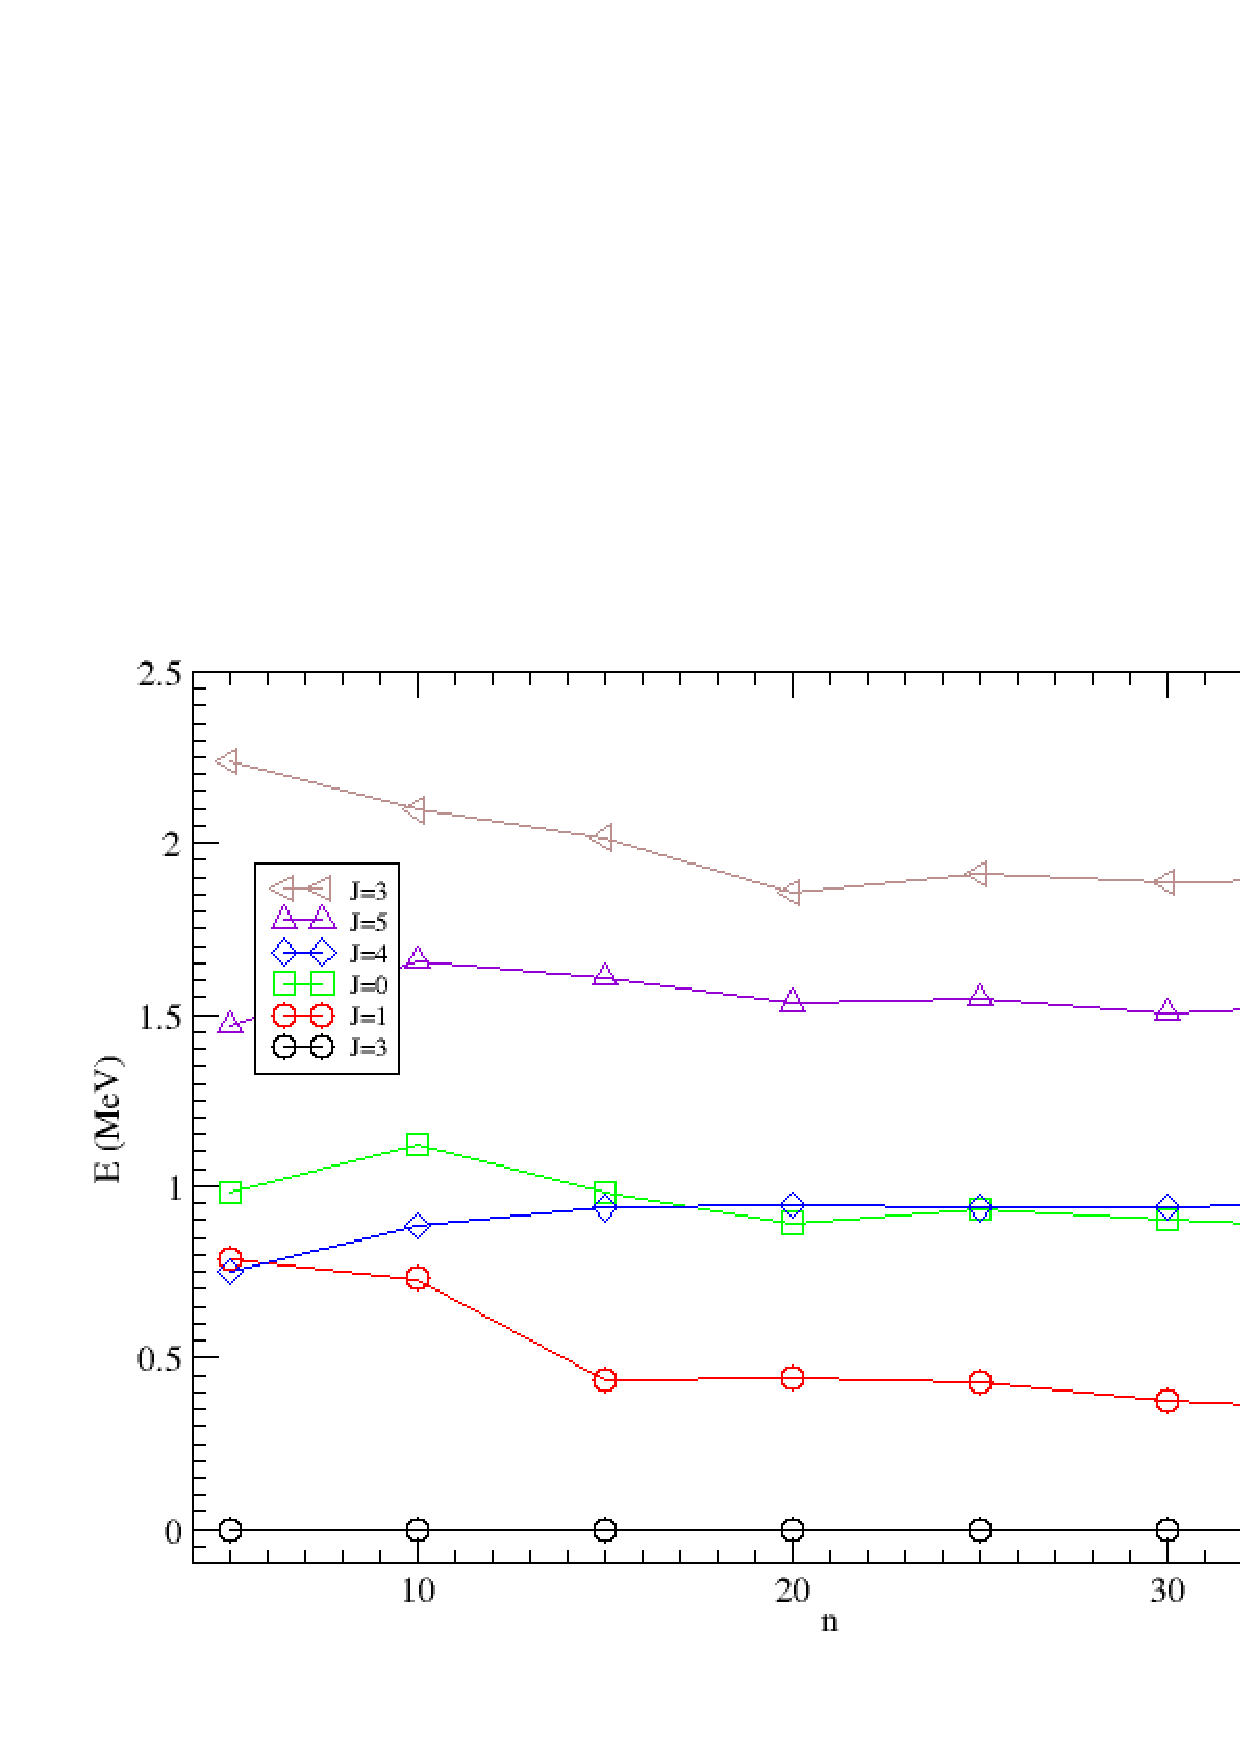
\includegraphics[width=.75\textwidth,clip]{Figures/pnism_ex_22na}
    \caption{$^{22}$Na low-lying excitation spectra as a function of $n$, the number of eigenstates retained from the pure proton and pure neutron
interactions used to form the basis. Here the maximum value of $n$ is $n=37$, when the entire basis is retained.}
    \label{22na}
\end{figure}
\begin{figure}
    \centering
    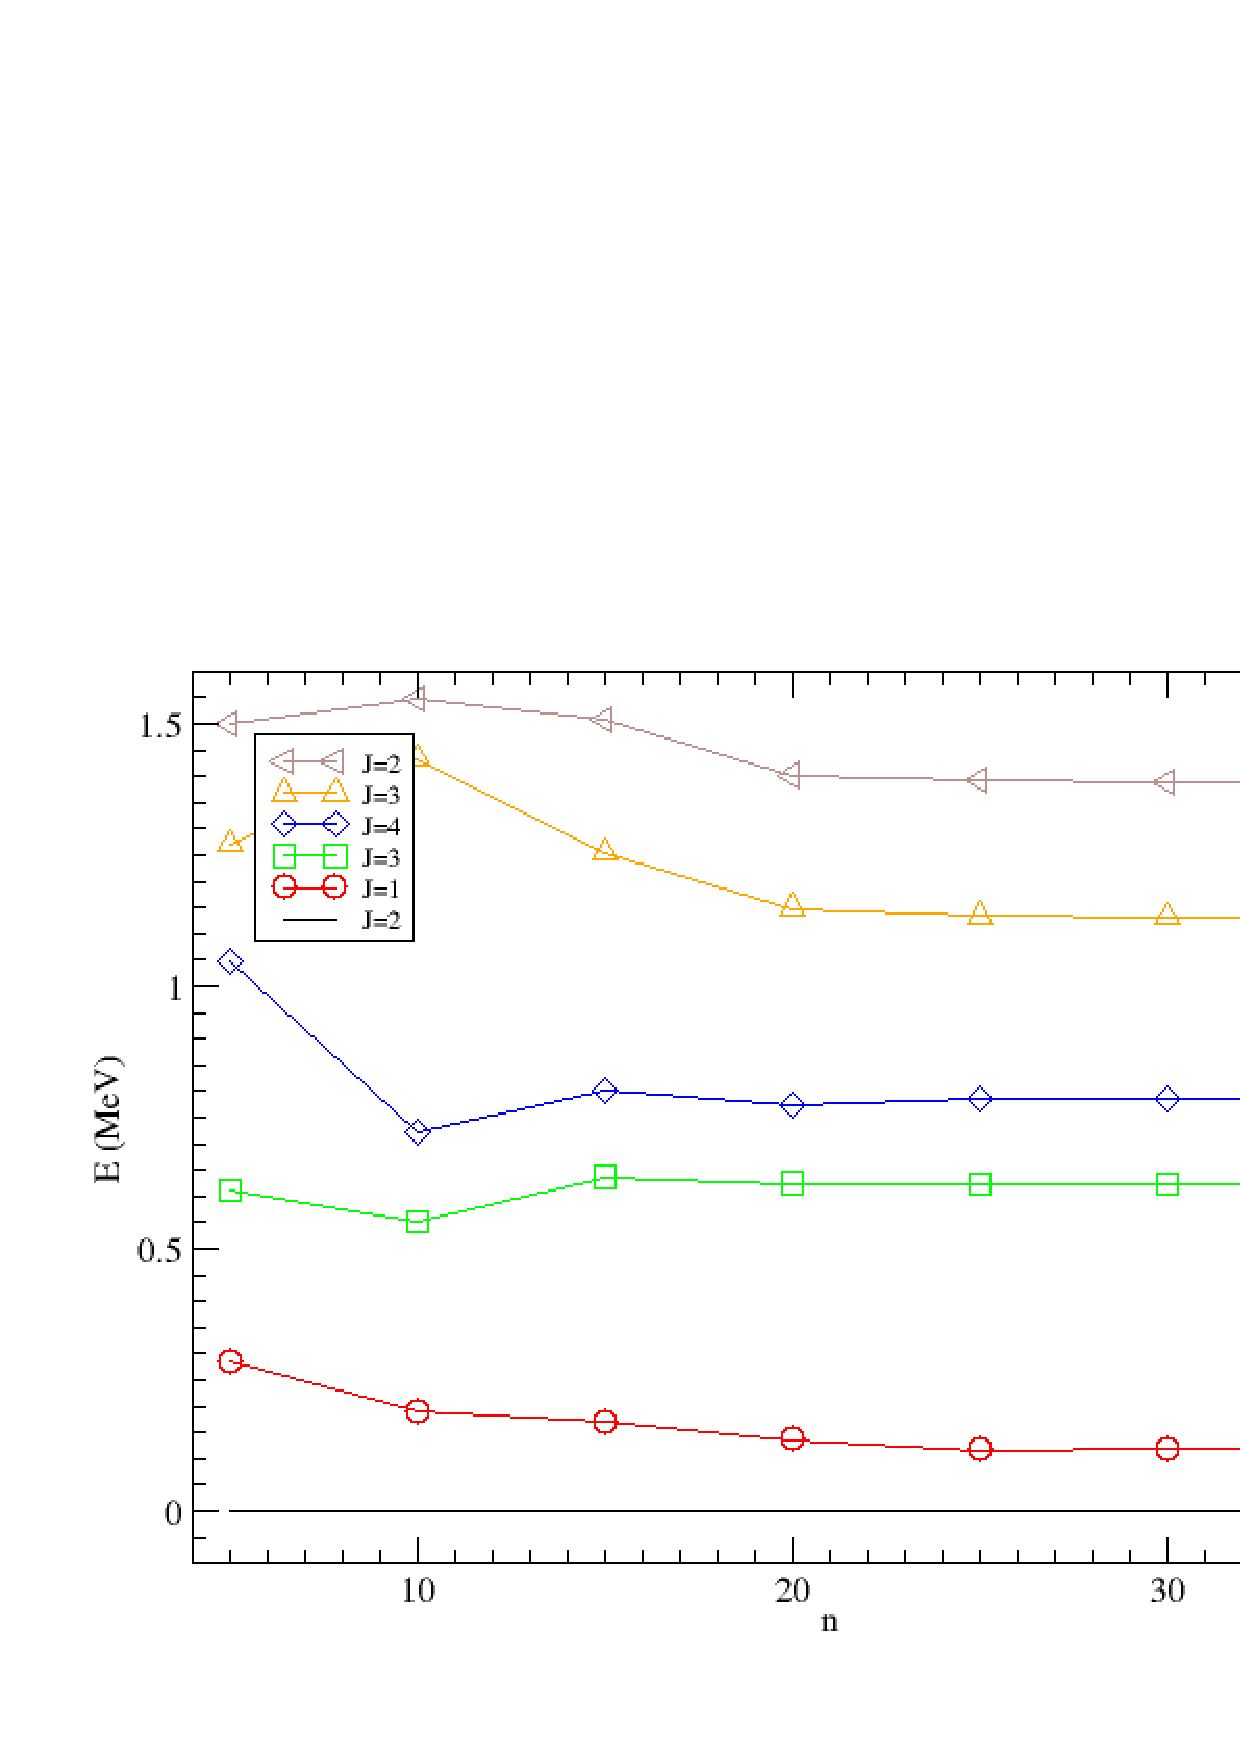
\includegraphics[width=.75\textwidth,clip]{Figures/pnism_ex_28na}
    \caption{$^{28}$Na low-lying excitation spectra as a function of the number of retained $n$. \boldmath$n_{max}=37$. Notice that $^{28}$Na
    converges faster than $^{22}$Na, while having the same basis dimensions.}
\end{figure}
\begin{figure}
    \centering
    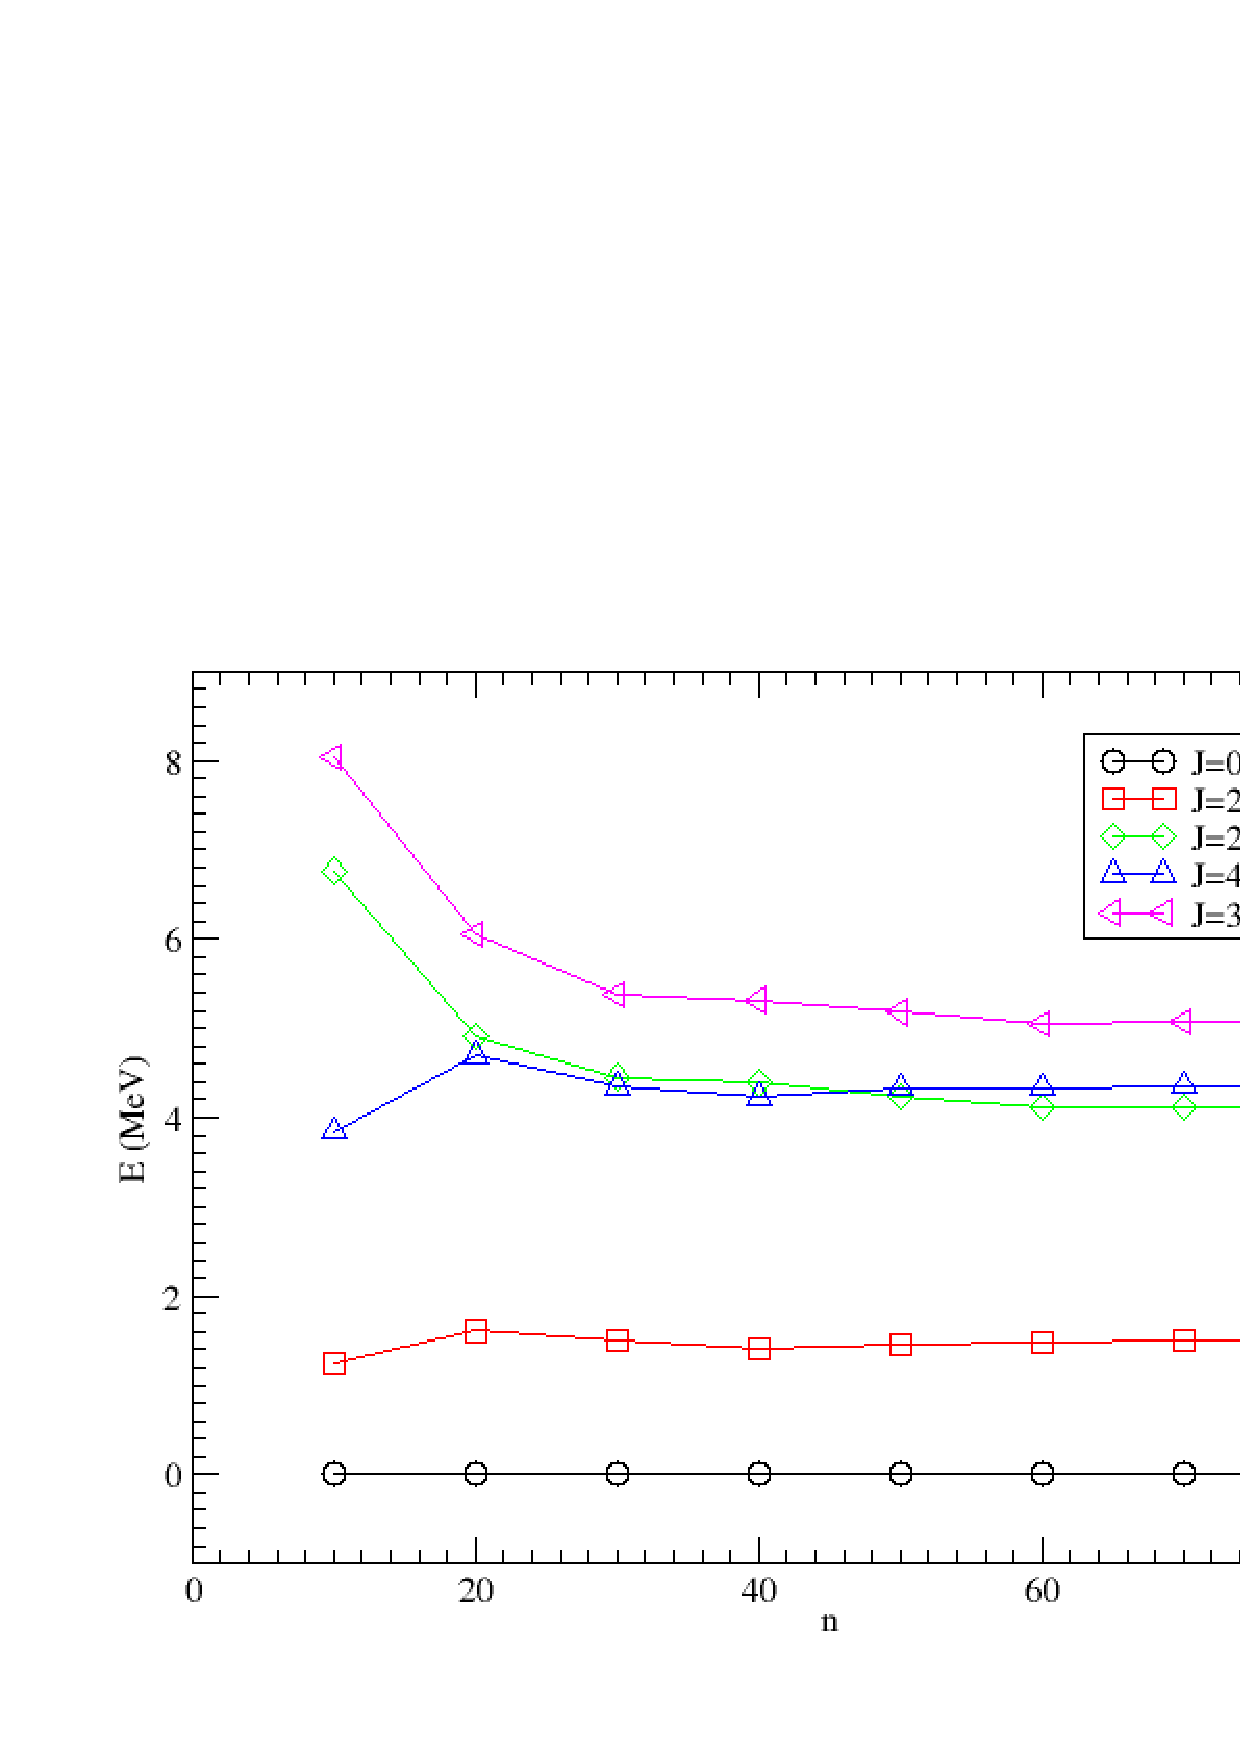
\includegraphics[width=.75\textwidth,clip]{Figures/pnism_ex_24mg}
    \caption{$^{24}$Mg low-lying excitation spectra. Symbols as in Figure \ref{22na}. Here \boldmath$n_{max}=81$.}
\end{figure}
\begin{figure}
    \centering
    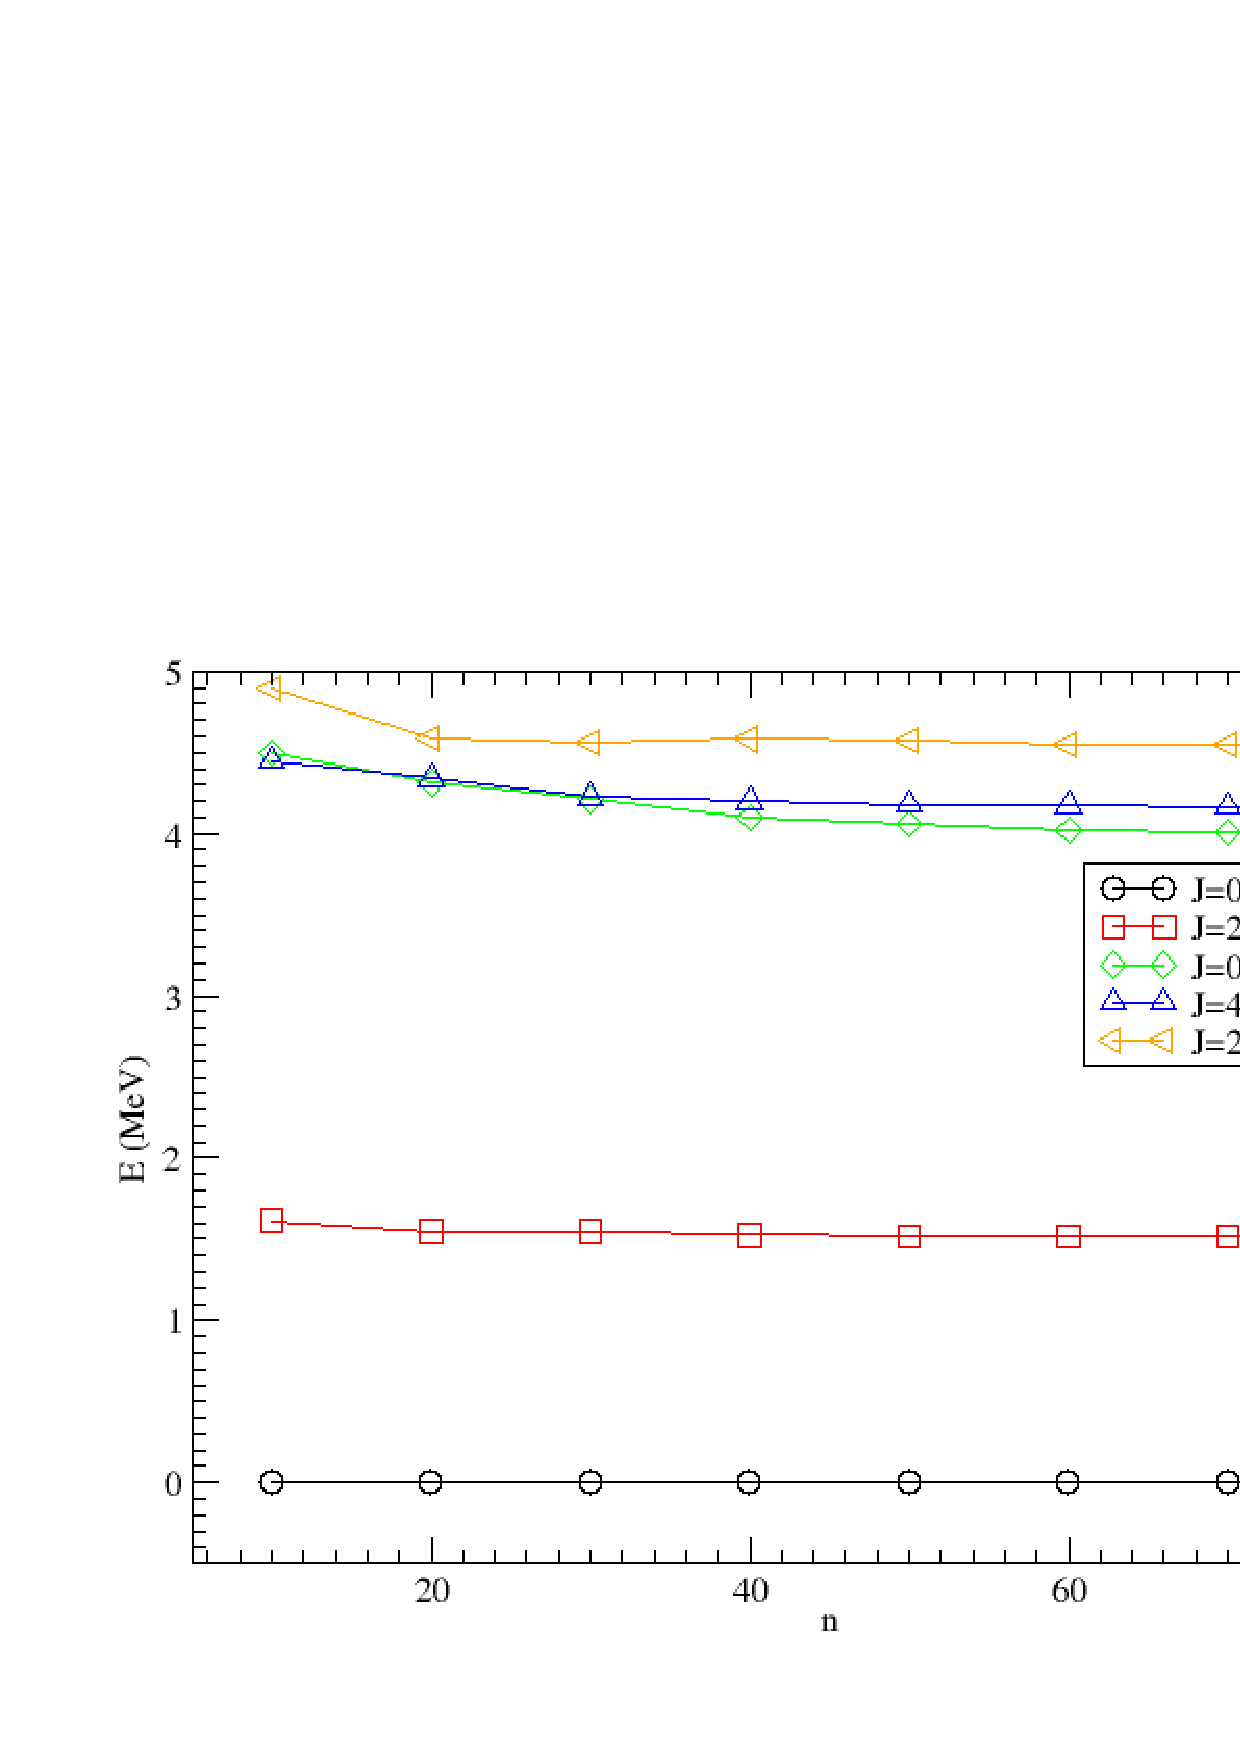
\includegraphics[width=.75\textwidth,clip]{Figures/pnism_ex_28mg}
    \caption{$^{28}$Mg low-lying excitation spectra. Symbols as in Figure \ref{22na}. \boldmath$n_{max}=81$ is the same as for $^{24}$Mg,
    but energies converge faster for $^{28}$Mg.}
\end{figure}
\begin{figure}
    \centering
    \includegraphics[width=.75\textwidth,clip]{Figures/E0_Ni56}
    \caption{$^{56}$Ni ground state energy convergence relative to complete basis wavefunction. }
\end{figure}
\begin{figure}
    \centering
    \includegraphics[width=.75\textwidth,clip]{Figures/Ni56}
    \caption{$^{56}$Ni low-lying excitation spectra. Unmarked curves are results from M-scheme calculation.}
\end{figure}
\begin{figure}
    \centering
    \includegraphics[width=.75\textwidth,clip]{Figures/E0_Ni60}
    \caption{$^{60}$Ni ground state energy convergence relative to complete basis wavefunctions as a function of the number of single-species basis states retained.}
\end{figure}
\begin{figure}
    \centering
    \includegraphics[width=.75\textwidth,clip]{Figures/Ni60}
    \caption{$^{60}$Ni low-lying excitation spectra. Unmarked curves are results from M-scheme.}
\end{figure}







\chapter{CONCLUSION AND FUTURE WORK}
\label{chap:conclusion}

This thesis was a study of proton-neutron entanglement entropy and the 
presentation of a new interaction shell model code, PNISM. It was shown 
that the proton-neutron entanglement entropy is inversely correlated
with the isospin of a atomic nuclei. 
This hypothesis was further supported by a decomposition of nuclear 
wavefunctions into pure proton and pure neutron eigenstates, which 
fall off exponentially. The fact that nuclei with greater isospin
appear to have weaker proton-neutron coupling suggests that heavier
nuclei with high isospin could be computed with even greater efficiency 
using this truncation scheme. 

We wrote a J-scheme interacting shell model code which takes proton wavefunctions
and neutron wavefunctions and creates a truncated basis of coupled proton
and neutron wavefunctions. The nuclear Hamiltonian is computed in this basis
and solved using standard numerical techniques. The ground state energy 
and wavefunctions converge exponentially to those of the full model space.
The results for three nuclei in the ($p_{1/2}$, $p_{3/2}$, $f_{5/2}$, $f_{7/2}$) model space, which would normally 
require a supercomputer to solve, were computed using PNISM running on 
a laptop. Results are not satisfactory and further research will need to be done to 
improve convergence. Eventually we would like be able to compute nuclei with full model
space dimensions in the billions using truncated model spaces in 
PNISM; however we are still working on some bugs to do with 
model spaces with more than one parity. 

In the future we will need to make changes to the code to improve convergence.
The model presented here is the simplest version in that basis states are
selected from the lowest eigenstates of the proton and neutron Hamiltonians.
This could be improved by introducing effective single-particle energies
to account for the contribution from the remaining states which were left out,
perhaps through some mean-field approximation.

In the current version, PNISM computes the entire set of Hamiltonian matrix
elements before diagonalizing. Memory utilization could be greatly improved
by diagonalizing the Hamiltonian after completing each value of total angular
momentum. This is possible since PNISM is a J-scheme code; matrix elements between states with
different total $J$ are independent. Here is a pseudo-code depiction of the current
procedure:
\begin{verbatim}
    DO J = JMIN, JMAX
        COMPUTE <AB,J| H |CD,J>
    END DO
    DO J = JMIN, JMAX
        DIAGONALIZE <AB,J| H |CD,J>
    END DO
    DEALLOCATE <AB,J| H |CD,J>
\end{verbatim}
The problem being that this requires storing the entire Hamiltonian in memory
before diagonalizing and writing to disk the much smaller set of truncated 
eigenstates and quantum numbers. If instead we use the following procedure:
\begin{verbatim}
    DO J = JMIN, JMAX
        COMPUTE <AB,J| H |CD,J>
        DIAGONALIZE <AB,J| H |CD,J>
        DEALLOCATE <AB,J| H |CD,J>
    END DO
\end{verbatim}
then we can expect a reduction in the total memory resources required by 
a factor that scales like the number of $J$ states required. While simple 
in principle, this will require a nontrivial restructuring of the 
code.

This reorganization of the code would also be compatible with a hybrid 
implementation of MPI\cite{mpi} and openMP\cite{openmp}. MPI is a 
distributed memory message passing interface commonly used for
parallelization. MPI will be called to distribute iterations
of the loop over $J$ values to various nodes of a cluster.
Each node, being assigned some allotment of work, will 
create numerous threads using openMP, a shared memory
multi-processing programming interface. If only one node is
available, then creation of openMP threads will be preferred.

% 
% The bibliography page, must be between main body and appendices
% 
% You must have thbib.bib file in the current directory 
% 
\bibliographystyle{aip}
\bibliography{thbib}


% This includes append.tex
\appendices
%\appendix
%
% If you only have one appendix, you should change the above to:
%\appendix
%
\chapter{Supplementary Notes}
\label{appendix: vc}
\section{Vector Coupling Coefficients}

Vector coupling coefficients, commonly referred to as Clebsch-Gordan coefficients
\cite{Shankar} are simply the coefficients of an expansion of a coupled angular 
momentum state with fixed total $J$ in a basis of coupled states 
$\ket{j_1m_1,j_2m_2}\equiv\ket{j_1m_1}\otimes\ket{j_2m_2}$. That is to say,
in the expansion
\begin{equation}
\ket{j_1j_2;JM}=\sum_{m_1m_2}\ket{j_1m_1,j_2m_2}\braket{j_1m_1,j_2m_2}{j_1j_2;JM},
\end{equation}
the inner products $\braket{j_1m_1,j_2m_2}{j_1j_2;JM}$ are the vector coupling
coefficients. This are often written as
\begin{equation}
    (j_1m_1j_2m_2|JM)\equiv \braket{j_1m_1,j_2m_2}{j_1j_2;JM}
\end{equation}
so that
\begin{equation}
    \ket{j_1j_2;JM} = \sum_{m_1m_2} (j_1m_1j_2m_2|JM) \ket{j_1m_1,j_2m_2}.
\end{equation}

\section{3-j Symbol}
An alternative to the vector-coupling coefficients are the so called three-J symbols
(3-j symbols). They are defined in terms of the vector coupling coefficients for the
coupling of three angular momenta\cite{Edmonds}:
\begin{equation}
    \begin{Bmatrix}j_1&j_2&j_3\\m_1&m_2&m_3\end{Bmatrix} \equiv
        (-1)^{j_1-j_2-m_2}(2j_2+1)^{-1/2}(j_1m_1j_2m_2|j_1j_2j_3-m-3).
\end{equation}

\section{6-j Symbols and 9-j Symbols}
Six-J and Nine-9 symbols are generalizations of vector coupling
coefficients which often appear in calculations involving complex angular
momentum algebra. I refer the reader to Edmonds\cite{Edmonds} for a complete description.

\section{Singular Value Decomposition}
\label{appendix: svd}
A singular value decomposition is a eigenvalue decomposition, 
generalized to non-square non-symmetric matrices. 
The method of singular value decomposition comes from a theorem 
which tells us that any $M \times N$ matrix A with $M \geq N$ can be written as
 the product of an $M \times N$ column-orthogonal matrix U, an $N \times N$ diagonal 
 matrix W with positive or zero elements (the singular values), and 
 the transpose of an $N \times N$ orthogonal matrix V\cite{NumRec}.
That is,
\begin{equation}
	A_{M \times N} = U_{M \times N} W_{N \times N} V_{N \times N}^T
\end{equation}
or in matrix notation,
\begin{equation}
	A_{ij} =  \sum_{a=1}^N U_{ia}  \sum_{b=1}^{N} W_{ab} V_{jb}
\end{equation}
Which, for the case where $M=N$, simply states that we can write a matrix $A$ as
a unitary transformation of a diagonal matrix containing the eigenvalues of $A$:
\begin{equation}
	A_{ij} = \sum_{ab}U_{ia}W_{ab}U_{jb}.
\end{equation}


\section{Lanczos Method}

This is an overview of the Lanczos method\cite{lanczos} used in this research. The 
Lanczos Algorithm is used to obtain the extremal eigenvalues of an $n \times n$
Hermitian matrix in $m<n$ linear operations. This is done by transforming the
Hermitian matrix into a truncated tridiagonal matrix containing the extremal 
eigenvalues,

\begin{equation}
    T = V^\dagger H V
\end{equation}

We begin with an $n \times n$ real-symmetric matrix $H$ and a fixed number $k<<n$
of iterations to carry out. Generate a random normalized vector $v(0)$ of dimension 
$n$ and carry out the following procedure:

\begin{verbatim}
    FOR all Lanczos iterations
        |w> = H|v(i)>
        a(i) = <v(i)|w>

        ! Orthogonalize against initial vector
        |w> = |w> - a(i)|v(i)>  

        IF (i>1), FOR all previous iterations
            ! Orthogonalize against prior vectors
            |w> = |w> - <v(j)|w>|v(j)> 

        b(i) = |w|
        |v(i+1)> = |w>/b(i)            
\end{verbatim}    

After $k$ iterations, the vectors $v(i)$ form the transformation matrix $V$ and
$a$ and $b$ contain the diagonal and subdiagonal elements of the tridiagonal 
matrix $T$.  

This algorithm can be used to extract the extremal eigenvalue and eigenvectors 
of $H$. By diagonalizing $T$, one can find $Tx = \lambda x$ where $x$ and $\lambda$
are the eigenvectors and eigenvalues of $T$. $H$ and $T$ are \textit{similar} matrices
and therefore have the same eigenvalues. Simultaneously $H\psi = \lambda \psi$ and 
$Tx = \lambda x$, so
\begin{equation}\begin{split}
    V^\dagger H Vx &= \lambda x \\
    VV^\dagger H Vx &= V\lambda x \\
    H Vx &= \lambda Vx, 
\end{split}\end{equation}
thus $\psi = Vx$ tells us how to obtain the eigenvectors of $H$ given the 
eigenvectors of $T$.

\section{Variational Principle}
\label{VP}
The Variational Principle is an extremely useful theorem in quantum mechanics as it
is the basis of many methods. 
The principle states that the expectation value of the Hamiltonian in any state is
greater than or equal to the expectation value of the Hamiltonian in the ground
state. Suppose we have a Hamiltonian $\hat{H}$ and an arbitrary state $\ket{\phi}$
both in some Hilbert space H. Because $\hat{H}$ is Hermitian, we are guaranteed
that it has a complete set of eigenvectors and eigenvalues, ${\ket{\psi}_i}$ and 
${E_i}$. Suppose that the lowest eigenstate has some, perhaps unknown, 
eigenvalue $E_0$. The Variational Principle is that the expectation value of 
$\hat{H}$ in the state $\ket{\phi}$ is
\begin{equation}
    \frac{\bra{\phi}\hat{H}\ket{\phi}}{\braket{\phi}{\phi}} \geq E_0.
\end{equation}
This is straightforward to prove since we can always write $\ket{\phi} = \sum_ic_i\ket{\psi}_i$.
Then equation (1) can be written
\begin{equation}\begin{split}
    \frac{\bra{\phi}\hat{H}\ket{\phi}}{\braket{\phi}{\phi}} &= 
    \frac{\sum_jc^*_j\bra{\psi}_j\hat{H}\sum_ic_i\ket{\psi}_i}{\sum_jc^*_j\bra{\psi}_j\sum_ic_i\ket{\psi}_i} \\
    &= \frac{\sum_{j,i}c^*_jc_i\bra{\psi}_j\hat{H}\ket{\psi}_i}{\sum_{j,i}c^*_jc_i\delta_{i,j}} \\
    &= \frac{1}{\sum_{i}|c_i|^2}\sum_{j,i}c^*_jc_iE_i\delta_{j,i} \\
    &= \frac{1}{\sum_{i}|c_i|^2}\sum_{j}|c_j|^2E_j
\end{split}\end{equation}
Since $E_0\leq E_i$ for all $i$, each term satisfies $|c_j|^2E_0\leq|c_j|^2E_j$ and
\begin{equation}
    \frac{1}{\sum_{i}|c_i|^2}\sum_{j}|c_j|^2E_j \geq \frac{1}{\sum_{i}|c_i|^2}E_0\sum_{j}|c_j|^2 \geq E_0.
\end{equation}
This inequality allows us to propose a model wavefunction and have the guarantee 
that our ground state will be bounded.




\chapter{Sample Density Matrix Files}
Here I have provided some redacted density matrix files to provide some context
for the discussion given on reading in density matrices. The following are data
from input files to be read into PNISM. The format of the density matrix files is
\begin{equation}
    \bra{Final\ State}[\pi^\dagger_a \pi_c]_{J_t}\ket{Initial\ State}
\end{equation}

These particle density matrix files are
used for calculating $^{20}$Ne in the sd model space with an inert $^{16}$O core. This means
that there are two valence protons and two valence neutrons. This first file
contains the excitation spectra and density matrices for a nuclei with
two protons and zero neutrons with $M=J_z=0$.
\begin{verbatim}
  BIGSTICK Version 7.8.1 Sept 2017
  single-particle file = sd
           2           0    <--- #protons, #neutrons
           0 +              <--- Jz, parity
  Time to compute jumps :    9.9999993108212948E-004
  Time to compute jumps :    0.0000000000000000     
  State      E        Ex         J      T 
    1    -11.77906   0.00000    -0.000   1.000
    2     -9.84945   1.92961     2.000   1.000
    3     -8.37591   3.40315     4.000   1.000
...
 Initial state #    2 E =   -9.84945 2xJ, 2xT =    4   2
 Final state   #    4 E =   -7.56341 2xJ, 2xT =    4   2
 Jt =   0, proton      neutron 
    1    1  -0.01892   0.00000
    2    2   0.45231   0.00000
    3    3  -0.75667   0.00000
 Jt =   2, proton      neutron 
    1    1  -0.01948   0.00000
    1    2   0.04273   0.00000
    1    3  -0.00230   0.00000
    2    1  -0.05930   0.00000
    2    2  -0.65142   0.00000
    2    3   0.40773   0.00000
    3    1  -0.03520   0.00000
    3    2  -0.71134   0.00000
 Jt =   4, proton      neutron 
    1    2   0.06297   0.00000
    2    1  -0.13163   0.00000
    2    2   0.08321   0.00000
...
\end{verbatim}
This second files contains the excitation spectra and density matrices for a nuclei with
two protons and zero neutrons with $M=J_z=1$. Notice that the states number labels
do not match up between the two files. The $M=J_z=1$ results are missing states
with $J=0$; you cannot have total angular momentum less than the z-component of
the angular momentum. Also notice that density matrix elements between the same
states (identified by $E$, $J$, and $T$ quantum numbers) are identical up to a 
phase. The $M=J_z=1$ density matrix file also has the entire set of $J_t$ quantum
numbers for a given initial and final state while the $M=J_z=1$ density matrix 
file is missing odd $J_t$ quantum numbers. Both solutions are required by PNISM
to obtain the entire density matrix.
\begin{verbatim}
  BIGSTICK Version 7.8.1 Sept 2017
  single-particle file = sd
           2           0
           2 +
  Time to compute jumps :    1.0000001639127731E-003
  Time to compute jumps :    0.0000000000000000     
  State      E        Ex         J      T 
    1     -9.84945   0.00000     2.000   1.000
    2     -8.37591   1.47354     4.000   1.000
    3     -7.56341   2.28605     2.000   1.000
...
Initial state #    1 E =   -9.84945 2xJ, 2xT =    4   2
 Final state   #    3 E =   -7.56341 2xJ, 2xT =    4   2
 Jt =   0, proton      neutron 
    1    1   0.01892   0.00000
    2    2  -0.45231   0.00000
    3    3   0.75667   0.00000
 Jt =   1, proton      neutron 
    1    1   0.01886   0.00000
    1    2  -0.03956   0.00000
    1    3   0.02182   0.00000
    2    1   0.00724   0.00000
    2    2   0.04334   0.00000
    3    1  -0.03337   0.00000
    3    3  -0.31605   0.00000
 Jt =   2, proton      neutron 
    1    1   0.01948   0.00000
    1    2  -0.04273   0.00000
    1    3   0.00230   0.00000
    2    1   0.05930   0.00000
    2    2   0.65142   0.00000
    2    3  -0.40773   0.00000
    3    1   0.03520   0.00000
    3    2   0.71134   0.00000
 Jt =   3, proton      neutron 
    1    1   0.02028   0.00000
    1    2  -0.03333   0.00000
    2    1   0.13226   0.00000
    2    2   0.75618   0.00000
    2    3   0.17724   0.00000
    3    2  -0.29377   0.00000
 Jt =   4, proton      neutron 
    1    2  -0.06297   0.00000
    2    1   0.13163   0.00000
    2    2  -0.08321   0.00000
...
\end{verbatim}















% 
% Make the library abstract page
% 
%\begin{libraryabstract}
  % This just inserts the the abstract.tex file
%  % You insert your abstract in the space below.




This thesis describes a nuclear shell model code which aims for a significant 
reduction in computer resource usage while 
retaining accuracy of results as compared to numerically exact solutions.
I begin with an introduction to the configuration interaction and shell
model calculations.
I then motivate the need for a proton-neutron decomposition of the Hamiltonian, and present
evidence for the viability of such a decomposition to reduce the size of the 
model space, through three different studies.  The first is a series of calculations of
proton-neutron entanglement entropy, a relatively novel approach in shell 
model calculations. Entanglement entropy measures the distribution
of wavefunction coefficients, and thus the viability of truncation
of a model space.
These calculations study the strength and origin of the 
isospin dependence of the proton-neutron entanglement entropy.
The second is a toy model that attempts to reproduce the entanglement entropy
properties of realistic nuclear calculations.
The third is a strength function decomposition of exact wavefunctions in 
an explicit proton-neutron formalism.
Finally, I discuss a code to calculate nuclear wave-functions by 
a coupling of proton and neutron wave-functions which are calculated beforehand 
by an existing interacting shell model code. 
Results and convergence properties of this code are provided and discussed.




%\end{libraryabstract}

\end{document}
